\documentclass[conference]{IEEEtran}
\IEEEoverridecommandlockouts
% The preceding line is only needed to identify funding in the first footnote. If that is unneeded, please comment it out.

\usepackage{cite}
\usepackage{amsmath,amssymb,amsfonts}
\usepackage{graphicx}
\usepackage{textcomp}
\usepackage{xcolor}
\usepackage[labelfont=bf, justification=justified]{caption}
\usepackage{subfig}
\usepackage{algorithm}
\usepackage{algpseudocode}
\usepackage{diagbox}
\usepackage{footnote}
\usepackage{bbding} %\Checkmark \XSolid
% to be able to draw some self-contained figs
\usepackage{tikz}
% inlined bib file
\usepackage{filecontents}
\usepackage{flushend}
\usepackage{xcolor}

\usepackage[most]{tcolorbox}
\newtcolorbox{highlighted}{colback=white,coltext=black,breakable,size=small}
\usepackage{lipsum}




\algrenewcommand\textproc{}% Used to be \textsc
\newcommand{\pushcode}[1][1]{\hskip\dimexpr#1\algorithmicindent\relax}

\def\BibTeX{{\rm B\kern-.05em{\sc i\kern-.025em b}\kern-.08em
    T\kern-.1667em\lower.7ex\hbox{E}\kern-.125emX}}
\begin{document}

\iffalse
\begin{frame}{\relax}%>>>

  \textbf{Response Letter}  


 \textbf{Major Changes:} 

  We appreciate the reviewers' and the meta-reviewer's comments and their efforts put into the reviews. To address the reviewers' concerns, we have prepared a revision with necessary changes addressing all the comments. 
  
  In summary, we have made the following major changes.
  
  First, we fixed some errors and further clarified the presentation, including correcting misuse of some terminologies pointed out by the reviewers and clarification of the concepts of "interactive" and "one-shot" transactions. We also improved the presentation about the motivation and contributions.
  
  Second, we made additional explanations to help readers understand the technical parts. For instance, we used an example to illustrate why 2PC over 2PL should not release locks before replicating the commit log if it wants to preserve linearizability. We provided a more detailed discussion about the timing of lock violation and how it fits in the two-phase commit message flow. We explained why DLV needs not to persist inter-transaction dependency on disks.
  
  Third, we conducted additional experiments to evaluate how different lock violation approaches affect transaction latency, the effects of lock violation on interactive transactions, and the cost of cascade abort.
  
  Fourth, we delete several contents to shorten the length of this paper. These contents include some tables, and knowledge unrelated to understand this paper.
  
  \begin{highlighted}
    We highlighted our changes  in boxed text in the revised manuscript.
  \end{highlighted}

 \textbf{Response to the meta reviewer’s comments:}

  \textbf{Comments}: Interesting paper on distributed lock management. The revision request is around presentation and missing explanations, like how RMs persist the dependency information, evaluating one-shot vs interactive, and analyzing the cascading aborts.
  
  \textbf{Response}: We added explanations to make these parts more understandable. We explained why DLV needs not to persist inter-transaction dependency on disks (the last paragraph of Section IV.B). We clarified the definitions of one-shot vs. interactive transactions (Section III.A and Fig. 3) and showed their relations with the DLV's design (Section IV.A).  We conducted additional experiments to evaluate the cost of cascading aborts (Section V.G).
  

  \textbf{Response to Reviewer 1’s comments:}

\textbf{W1}. The paper does not give enough explanations to some important concepts and techniques which are necessary for readers to understand the design of DLV.

\textbf{Response}: We made additional explanations to make the technical parts more understandable. We clarified the definitions of one-shot vs. interactive transactions (Section III.A and Fig. 3). We showed why 2PC over 2PL should not release locks before replicating the commit log to preserve linearizability (Section I, Page 2, 2nd paragraph). We provided more deals of the different DLV designs (Section IV.A). We explained why DLV needs not to persist inter-transaction dependency on disks (the last paragraph of Section IV.B).

\textbf{W2}. The paper does not discuss and prove how RMs persist dependency information and achieve fault-tolerance.

\textbf{Response}: Persisting dependency information will introduce additional overhead. DLV chooses not to persist dependency information in stable storage. In DLV, each RM independently maintains its dependency information locally in memory. (If two transactions conflict on an RM, their dependency introduced by the conflict will be recorded only in that RM.) When a node fails, the dependency information on the node can all be discarded. If a transaction’s in value on an RM is greater than 0, we can guarantee that this RM has not entered the uncertain “prepare commit” state. Upon a failure, this un-prepared RM can simply vote to rollback the transaction without referring to the dependency information. Otherwise, if the RM is already prepared, we do not need the in value to proceed. Therefore, it is safe to discard the dependency information when a failure occurs. We have added this part of explanation to Section IV.B.

\textbf{W3}. The experiment part does not show transaction latency, which could be interesting for readers, since DLV is mainly used to shorten the lock blocking time.

\textbf{Response}: In fact, DLV does not necessarily benefit transaction latency. Although it has shortened the lock blocking time, a transaction still needs to hold until all its preceding transactions end. This final wait phase is necessary to ensure transactions' correctness. We have added a set of experiments to evaluate the effects of DLV on transaction latency (Section V.H). It shows that latency is more affected by the system's saturation level rather than by lock violation.

\textbf{D1}. The first main contribution of this paper says that “CLV does not necessarily help in enhancing the performance of GDDB”. But (a) the paper has only a little explanation about what CLV is in the Related Work, which is not enough to be a main contribution; (b) It proposed DLV as a variation of CLV, but not clearly explain the differences between them; (c) it has no experiments to support the claim.

\textbf{Response}: We added more discussion about CLV and how to apply it to distributed databases (Section II.B). We also clarified the description of our contributions accordingly(Section I).

\textbf{D2}. The definitions of one-shot and interactive transactions are not clear. The paper does not explain (1) why they summarize these two types of transactions, (2) why their message flows are different and what features the transaction has to make the difference, (3) why it is necessary to do so. And there are no experiments comparing

\textbf{Response}: In the previous version, interactive and one-shot transactions were not clearly defined. In the revised version (Section III.A), we used a different pair of terminology to classify the transactions and explained why they are related to our design choices. 
Basically, if a transaction knows that it will not violate serializability before issuing the prepare message, it is a DP (deterministic prepared) transaction. Otherwise, it is an NDP (non-deterministic prepared) transaction. In a DP transaction, if an RM receives a prepare message, it knows that other RMs of this transaction will all be prepared sooner or later, as long as there is no failure. In practice, most interactive transactions can be categorized as DP transactions, but not all. Fig. 3 in the revised version illustrates the difference. The distinction between DP and NDP will affect how DLV conducts lock violation and dependency tracing when an RM receives a prepare message. (In principle, it only affects the designs of DLV1 and DLV1x.)
We have conducted an additional evaluation on interactive transactions (DP transactions) (Section V.F).

\textbf{D3}. The message flow in Figure 8 is not so clear. It is better to mark which phase of 2PC the message is for. And the paper does not explain how the serializability test message sending from RMs to TM comes.

\textbf{Response}: We had marked the message type in the figure. We have also added some explanation on how the serializability test is issued and what it is used for (Section IV.A and Fig. 8).

\textbf{D4}. The paper let RM nodes maintain the dependency information, but does not explain how it is persisted to achieve fault tolerance.

\textbf{Response}: See our response to W2.


\textbf{Response to Reviewer 2’s comments:}

\textbf{W1}. The only minor concern I have is that the techniques are fairly straightforward extensions of existing lock violation ideas from centralized databases. But I believe the paper sufficiently compensates for this by thoroughly exploring these ideas in a new context. I enjoyed reading the technical discussion and the experiments.

\textbf{Response}: This is quite right. We applied the old idea of lock violation to geo-replicated distributed database. Nevertheless, we presented and evaluated different lock violation approaches on GPDB, and some results are not trivial. We hope our results and insights can be helpful to future developers of distributed database systems.

\textbf{W2}. I would like to see a discussion how a GDDB or DB admin would select the best DLV option for their application. How can this be decided automatically? From the experiments, it looks like DLV1x is the winner. Does this generalize to other applications?

\textbf{Response}: The evaluations show that early lock violation fails to scale when the degree of concurrency is high. It also performs worse in handling workload with high abort rates. However, it can achieve good performance when the system is not saturated. In contrast, late lock violation is more adaptive to various workloads and scales well. 
Automatically deciding DLV scheme to use sounds like a good idea. We believe such automation is possible, while it requires a lot of work. This can be an interesting topic for future research.

\textbf{D1}: There really is not much else to be said, except for a few typos. Here are some examples: Sec II.B "This has been illustrated in Fig. 1." should reference Fig. 2 instead. Sec IV.A "...unless it performs a serializability test as DLV1 does." should refer to DLV1x. Sec V.C "400,00 rows" should probably be 400,000 rows.

\textbf{Response}: Thanks for pointing out the errors. We have fixed them. We also went through the paper and fixed a few other errors and typos. 

\textbf{Response to Reviewer 3’s comments:}

\textbf{W1}. I would appreciate more analysis on cascading aborts.

\textbf{Response}: We have added an experimental study on cascading aborts (Section V.G). Cascade abort seldom occurs for late lock violation, as it violates lock after the transaction finishes its work successfully. Early lock violation is more vulnerable to cascade abort. Nevertheless, our experiment results showed that, even in early lock violation, cascade aborts constituted only a small proportion of the actual aborts. We believe that in general cases, such as TPC-C, cascade aborts will not be a serious threat to the performance.

\textbf{W2}. There is no evaluation of one-shot vs. interactive.

\textbf{Response}: In the revision, we refined our definitions of one-shot and interactive transactions (Section III.A). We also included an additional experimental study on interactive transactions (Section V.F).

\textbf{D1}. I don't quite understand the ``one-shot" execution in this paper. My understanding of ``one-shot" is that the user provides all the input parameters at the beginning of the transaction so there is no further interaction between the database and the user before commit/abort. The ``one-shot" execution in this paper seems different: the TM immediately starts the 2PC process without reading data from RMs beforehand. This does not seem to work if the transaction contains complex logic; for example, the data to write depends on some values read. Please clarify the use case the "one-shot" execution here. 

\textbf{Response}: Thanks for pointing this out. There was some misuse of one-shot transactions and interactive transactions in the previous version.
In the revised version (Section III.A), we used a different pair of terminology to classify the transactions and explained why they are related to our design choices. Basically, if a transaction knows that it will not violate serializability before issuing the prepare message, it is a DP (deterministic prepared) transaction. Otherwise, it is an NDP (non-deterministic prepared) transaction. In a DP transaction, if an RM receives a prepare message, it knows that other RMs of this transaction will all be prepared sooner or later, as long as there is no failure. In practice, most interactive transactions can be categorized as DP transactions, but not all. Fig. 3 in the revised version illustrates the difference. The distinction between DP and NDP will affect how DLV conducts lock violation and dependency tracing when an RM receives a prepare message.

\textbf{D2}. Related to D1, in the evaluation section, are the transactions modeled as "one-shot" or "interactive"? Would these two models lead to different design decisions?

\textbf{Response}: We included an additional experimental study on interactive transactions (DP transactions) (Section V.F). We showed that DLV1 and DLV1x demonstrate similar performance in interactive transactions, as they tend to violate locks at the same stage. This is quite different from the results in NDP transactions.

\textbf{D3}. Please consider flipping the order of Figures 9 and 10. They appear in the opposite order in paper.

\textbf{Response}: We corrected the order in the revised paper.

\textbf{D4}. Please report some analysis on cascading aborts. For example, what percentage of aborts are caused by cascading aborts? What is the main cause of cascading aborts? (e.g., detected deadlocks or aborts due to WaitDie) Would different variants of DLV lead to different numbers of cascading aborts?

\textbf{Response}: Please refer to our response to W1. As our experimental results show, cascade aborts are more likely to be triggered by active aborts, e.g., aborts caused by accessing non-existent data. 

\textbf{D5}. This last comment is more like a question rather than an evaluation comment: In Fig 2, why does the locking critical path end after RM finishes logging? I thought it could end when the RM receives the commit request from the TM. Because at that point, the transaction is already destined to commit.

\textbf{Response}: We added an example in Section I (Page 2, 2nd paragraph) to explain why it is necessary to preserve locks until the commit log is replicated. We showed that 2PC over 2PL might violate linearizability if it releases locks before replicating the commit log. While serializability and recoverability can in theory be preserved even if we release lock earlier, we may not be willing to sacrifice linearizability, as it is often desired by applications .


\end{frame}%<<<

\fi 

\title{Lock Violation for Fault-tolerant Distributed Database System*\\
\thanks{This work was supported by Alibaba Group through Alibaba Innovative Research (AIR) Program. This work was partially supported by the NSFC Project No. 61772202.
}
}


\author{\IEEEauthorblockN{Hua Guo}
\IEEEauthorblockA{\textit{School of Information} \\
\textit{Renmin University of China}\\
Beijing, China \\
guohua2016@ruc.edu.cn}
\and
\IEEEauthorblockN{Xuan Zhou}
\IEEEauthorblockA{
\textit{Shanghai Engineering Research Center of Big Data Management} \\
\textit{East China Normal University}\\
Shanghai, China \\
xzhou@dase.ecnu.edu.cn}
\and
\IEEEauthorblockN{Le Cai}
\IEEEauthorblockA{
%\textit{} \\
\textit{Alibaba Group}\\
San Mateo, CA, US \\
le.cai@alibaba-inc.com}
}

\maketitle

\begin{abstract}
Modern distributed database systems scale horizontally by partitioning their data across a large number of nodes.
Most such systems build their transactional layers on a replication layer,
employing a consensus protocol to ensure data consistency to achieve fault tolerance.
Synchronization among replicated state machines thus becomes a significant overhead of transaction processing.
Without careful design, synchronization could amplify transactions' lock duration and impair the system's scalability.
Speculative techniques, such as Controlled Lock Violation (CLV) and Early Lock Release (ELR), prove useful in shortening lock's critical path and boosting transaction processing performance.
To use these techniques to optimize geo-replicated distributed databases(GDDB) is an intuitive idea.  
This paper shows that a naive application of speculation is often unhelpful in a distributed environment.
Instead, we introduce Distributed Lock Violation (DLV), a specialized speculative technique for geo-replicated distributed databases.
DLV can achieve good performance without incurring severe side effects.
\end{abstract}

\begin{IEEEkeywords}
Distributed Database, Transaction, Locking, High Availability
\end{IEEEkeywords}

\section{Introduction}

Modern distributed database systems scale-out by partitioning data across multiple servers,
so as to increase throughput by running transactions in parallel.
When a transaction needs to access multiple partitions, it has to employ a coordination protocol to ensure atomicity.
Such distributed transactions may lead to significant performance degradation, mainly due to the two reasons\cite{Calvin:conf/sigmod/ThomsonDWRSA12}:
1. Coordinated commit requires a chatty protocol, such as Two-Phase Commit (2PC), which introduces tremendous network overheads;
2. Message transmission overlaps with the critical path of transaction commit, which worsens the contention among transactions.

These performance issues can be more severe for geo-replicated databases.
The replication layer of a geo-replicated database often uses a Paxos-like consensus protocol to ensure consistency among replicas.
Replication and consensus introduce an additional amount of message transmission, which further increases the duration of transactions.


\begin{figure}[tbp]
  \centerline{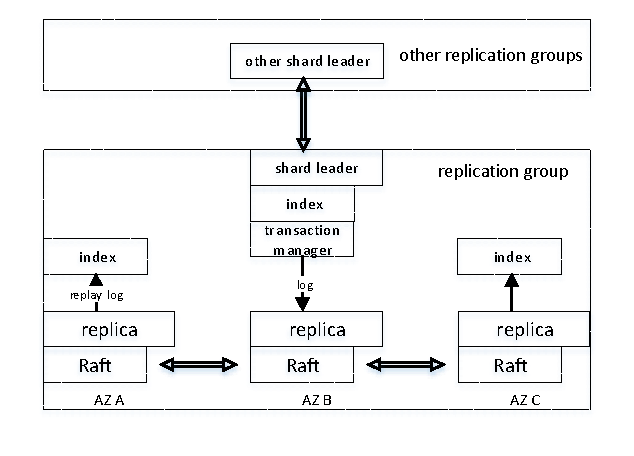
\includegraphics[scale=0.7]{architecture.pdf}}
  \caption{Typical architecture of GDDB}
  \label{fig:architecture}
\end{figure}

Fig.~\ref{fig:architecture} presents a typical architecture of a geo-replicated distributed database (GDDB).
Data are partitioned into many chunks.
Each chunk is replicated to several Availability Zones (AZ) \cite{Aurora:conf/sigmod/VerbitskiGSCGBM18}.
Among the available zones, the replication layer employs a consensus protocol to shield data consistency.

As discussed in some previous works \cite{Calvin:conf/sigmod/ThomsonDWRSA12}\cite{Tapir:conf/sosp/ZhangSSKP15}\cite{Janus:conf/osdi/MuNLL16},
this architecture has to rely on a two-layer protocol (which integrates the commit protocol and the consensus protocol) to ensure transactions' correctness.
It may fail to scale when confronted with a highly contended workload.


\begin{figure}[tbp]
  \centerline{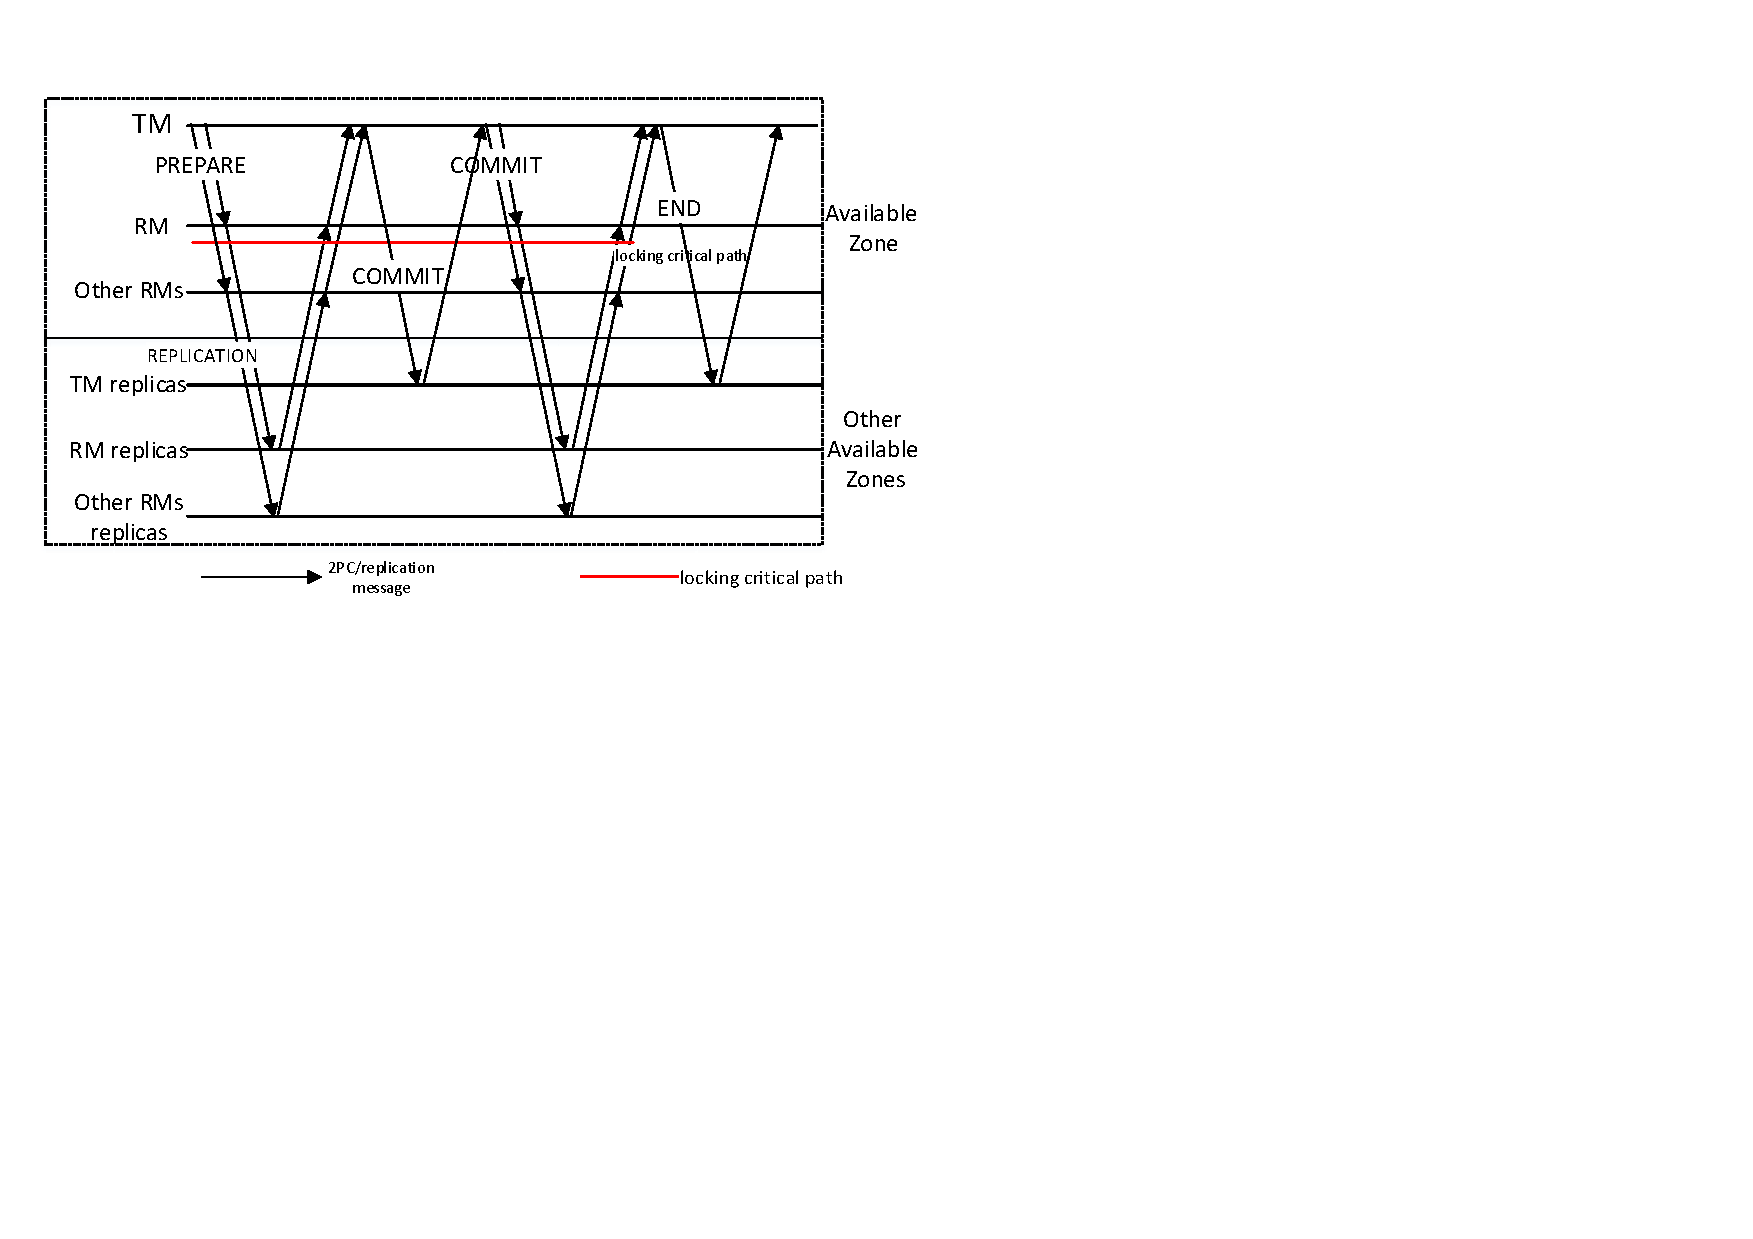
\includegraphics[scale=0.50]{message_flow.pdf}}
  \caption
  {
The DB uses S2PL for concurrency control and uses 2PC protocol as the atomic commit protocol.
This figure shows the message flow of a transaction commit.
The red lines represent the critical paths of locking.
    }
\label{fig:message_flow}
\end{figure}

Fig.~\ref{fig:message_flow} shows the message flow of a distributed transaction in such an architecture. We assume that
GDDB uses Strict Two-Phase Locking (S2PL) for concurrency control and 2PC as the commit protocol, and the replication layer works over a Wide Area Network (WAN).
When a transaction requests to commit, the \emph{TM (transaction manager)} issues a `prepare' message to each \emph{RM (resource manager)}.
Then, each \emph{RM} replicates its vote (`prepare commit' or `prepare abort') to its replicas through a consensus protocol before it
sends its voting result to \emph{TM}.
After the \emph{TM} collects all the votes from the \emph{RMs}, it first replicates its decision (`commit' or `abort') to its replicas before broadcasting the decision to all the \emph{RMs}.
Once a \emph{RM} receives the final decision from the \emph{TM}, it also needs to replicate the log to the corresponding replicas.
Only at this moment can the GDDB reach a consensus about commit or abort.
Then, the \emph{RM} can release the locks it had retained over the accessed data.
Finally, \emph{TM} replicate an `end' log to finish the transaction and clean the transaction context.
%\begin{highlighted}



In a replicated DB, if a \emph{RM} releases its locks immediately after receiving the commit message before persisting its decision, linearizability may not be guaranteed, although transactions can ensure serializability.
The following is a situation:
(1) A \emph{RM} of a transaction ${T}$ receives a commit message.
(2) The \emph{RM} releases ${T}$'s lock on a tuple ${x}$. Following that,
a second transaction ${R}$ reads ${T}$'s write on ${x}$ and commits successfully.
(3) Before the \emph{RM} persists its commit log, the node which it resides on fails. 
(4) After the node recovers, the \emph{RM} re-enters an uncertain state, as it cannot remember it has received a commit message. At this time, the \emph{RM} of ${T}$ needs to wait for an additional commit message from ${T}$'s \emph{TM} to recovery its committed state.
A third transaction ${S}$ cannot read the new version of ${x}$,
but transaction ${R}$ had read ${x}$'s new version successfully, which may violate linearizability.
%\end{highlighted}

%\begin{highlighted}
Lock duration of transaction commit in such an architecture, i.e., the red line in Fig.~\ref{fig:message_flow}, involves multiple messages round trips over the WAN.
And there were also messages between LAN.
Different network environment has various RTT(round trip time).
Take Alibaba ECS servers as an example.
The RTT between two servers in the same AZ is about 0.12ms, and the RTT in the different AZs of the same cities is 1.96ms.
RTT of servers in different cities of the same continents can be 33.5ms(from Hangzhou to Heyuan).
On different continents, the RTT could be 98.6ms(from Virginia to Frankfurt), 206ms(from Hangzhou to Frankfurt).
Geo-replication can remarkably amplify lock duration and worsen the contention among transactions.
Consider that the RRT over a geo-distributed WAN is around 30-200 milliseconds during a transaction. 
This vast difference of RTT between WAN and LAN lets us consider exploiting the speculative technique to reduce lock blocking.
%\end{highlighted}
Speculative techniques, such as Early Lock Release (ELR) \cite{EfficientLocking:conf/vldb/KimuraGK12} and Controlled Lock Violation (CLV)
\cite{CLV:conf/sigmod/GraefeLKTV13}, prove to be effective in optimizing centralized transaction processing.
They aim at improving concurrency by excluding data persistence (i.e., logging) from lock duration.
In a GDDB, data synchronization among replicas can be treated as prolonged data persistence, which needs to ship and persist logs on the majority of replicas.
This gap inspires us to exploit speculation to shorten lock duration in GDDB.

However, the application of speculation in a distributed environment is complex.
For instance, when working with 2PC, we need to decide to violate (or release) lock at which phase.
As some previous work suggested \cite{CLV:conf/sigmod/GraefeLKTV13}, lock violation at an early phase may enable a higher degree of concurrency,
while it may face excessive overheads of dependency tracing or cascade abort.
On the contrary, lock violation at a late phase costs less on dependency tracing and cascade abort,
while it may lose the opportunity of harnessing more concurrency.

Moreover, not all transactions can benefit from CLV or ELR, e.g., workload with little conflict.
It is unnecessary and even harmful to apply speculation to all cases.

The contribution of this paper can be summarized as follows:

%\begin{highlighted}
  

1. To the best of our knowledge, this is the first study of the speculation method(e.g., CLV) on GDDB.
We found that there is no straightforward way to extend existing lock violation techniques to GDDB. 
There are many design choices, and their performance on GDDB is unknown. 
Cascade abort, dependency tracing, deadlock handling, and storage implementation need to be considered to construct a holistic solution.  

2 We propose a technique called Distributed Lock Violation(DLV)  to enhance the performance of GDDB.
DLV considers several different time windows to perform lock violation.
Based on the timing of lock violation, DLV adopts different methods of dependency tracing and deadlock handling accordingly to minimize the overheads.
We evaluated the different design choices of DLV and obtained a generalization about their best application scenarios, respectively.
%\end{highlighted}

We organized the remainder of this paper as follows.
Section \ref{sec:relate_work} reviews the related work.
In Section \ref{sec:non_strict} we explain lock violation and how to ensure the correctness of distributed transactions handling lock violation.
Section \ref{sec:implement} introduces our design of DLV.
Section \ref{sec:experiment} evaluates DLV and compares it against other forms of lock violation.
Section \ref{sec:conclusion} concludes this paper.


\section{Relate Work}
\label{sec:relate_work}
%This section introduces the related work of this paper.

\subsection{Transaction Processing on Replicated Databases}


Most replicated databases rely on state-machine replication (SMR) to realize high availability.
SMR often uses a consensus protocol to synchronize replicas.
The synchronization introduces a significant amount of network traffic and becomes a significant overhead of replicated database systems.
Paxos~\cite{Paxos:journals/tocs/Lamport98} is the most well-known consensus protocol.
Raft\cite{Raft:conf/usenix/OngaroO14} is a similar consensus protocol to Paxos.
Google Spanner \cite{Spanner:conf/osdi/CorbettDEFFFGGHHHKKLLMMNQRRSSTWW12},
NuoDB \cite{NuoDB}, CockroachDB \cite{CockroachDB} and TiDB \cite{TiDB} are all geo-replicated DBMSes built upon Paxos or Raft.
They all face heavy costs incurred by data synchronization and consensus.

Previous work has proposed many techniques
to minimize the cost of synchronization.
VoltDB \cite{VoltDB} and Calvin \cite{Calvin:conf/sigmod/ThomsonDWRSA12} employ a deterministic transaction model
to reduce the coordination cost of distributed transactions.
A deterministic scheduler enables active replication, allowing transactions to kick off synchronization at the earliest possible time.
Tapir \cite{Tapir:conf/sosp/ZhangSSKP15} relaxes the replication layer's consistency requirements so that it can reduce the message round trips to reach consensus.
Janus \cite{Janus:conf/osdi/MuNLL16} aims to minimize wide-area message round trips
by consolidating the concurrency control mechanism and the consensus protocol.
It uses deterministic serializable graph tracing to ensure the atomicity of transactions.
In a nutshell, Tapir and Janus both co-designed the transaction and replication layers of distributed databases so that they only need to incur one wide-area message round trip to commit a transaction.
However, VoltDB, Calvin, Tapir, and Janus all impose strict constraints on implementing the transaction layer, making them incompatible with existing systems, such as Spanner and CockroachDB.
In contrast, our work focuses on the optimization opportunities, in particular lock violation, in a general implementation of geo-replicated distributed databases (GDDB), as depicted in Fig.~\ref{fig:architecture}.

\subsection{Optimization on Locking based Concurrency Control}
Two-phase locking (2PL) is the most widely used concurrency control mechanism.
As a pessimistic method, 2PL assumes a high likelihood of transaction conflict.
It uses locks to enforce the order of conflicting transactions.
Strict 2PL (S2PL) is a brute force implementation of 2PL.
It requires a transaction to preserve all its locks until it ends.
As S2PL can easily guarantee transactions' recoverability, many databases choose to use it.
When extending S2PL to GDDB, transaction commitment and replication would substantially enlarge the lock blocking time,
as the commitment will involve several message round trips. 
This time has been illustrated in Fig.~\ref{fig:message_flow}.

All S2PL implementations adopt a specific approach to resolve deadlocks.
While deadlock detection proves effective in centralized database systems \cite{MySQL}\cite{PostgreSQL}, it is costly in a distributed environment.
In the \emph{no-wait}
\cite{EvaluationOfCC:journals/pvldb/HardingAPS17}
approach, a transaction immediately aborts if it fails to place a lock.
Previous works showed that this is a scalable approach in a distributed environment \cite{EvaluationCC1000Cores:journals/pvldb/YuBPDS14}\cite{EvaluationOfCC:journals/pvldb/HardingAPS17},
as it eliminates blocking completely.
However, it poorly performs when dealing with a high-contention workload.
Another approach is \emph{wait-die} \cite{LockNoWait:journals/csur/BernsteinG81}.
It avoids some false-positive aborts encountered by \emph{no-wait} by utilizing timestamps.
The \emph{deadlock detection} approach \cite{LockCC:conf/ds/GrayLPT76} detects deadlock by explicitly tracing wait-for relationship among transactions
In this work, we discuss and evaluate both the \emph{wait-die} deadlock prevention and deadlock detection approaches.


We can use the speculation technique to optimize the performance of locking-based concurrency control.
Early lock release (ELR)
\cite{EfficientLocking:conf/vldb/KimuraGK12}
\cite{ELR:dewitt_implementation_1984}
\cite{PS2PL:conf/icdt/Soisalon-SoininenY95}
\cite{Aether:journals/pvldb/JohnsonPSAA10}
\cite{Actor-Oriented-DB:conf/icde/Bernstein18}
is a typical speculative technique.
ELR allows a transaction to release its locks before DB flush its commit log to disk.
It was first proposed by DeWitt et al.\cite{ELR:dewitt_implementation_1984}.
Soisalon-Soininen et al. \cite{PS2PL:conf/icdt/Soisalon-SoininenY95} analyzed its correctness in various settings.
Many other works applied and evaluated ELR in different types of systems
\cite{EfficientLocking:conf/vldb/KimuraGK12}
\cite{Aether:journals/pvldb/JohnsonPSAA10}.


%\begin{highlighted}

CLV further advanced ELR. 
It is more straightforward, more robust, and more precise than ELR.
By definition, ELR  applies only to the second phase of 2PC, while CLV applies to both phases.
In this sense, CLV is more related to our work.

Although CLV can be extended to work with distributed systems, 
how to use lock violation to empower distributed transactions remains a challenge.
CLV adopts a Register and Report (RARA) approach \cite{HeckatonMVCC:journals/pvldb/LarsonBDFPZ11} to trace dependencies among transactions.
RARA works well on a centralized database. 
However, in a distributed environment, dependency tracing becomes much more costly.
Cascade abort is another challenge for lock violation. 
Excessive cascade aborts can lead to severe performance downgrade.
Handling deadlock in a distributed environment is also challenging. It is not apparent what is the good way to deal with deadlock when lock violation is applied.
Moreover, there are different timings for performing lock violation in a GRDB. Selection of the best timing is an unexplored topic.
  
%\end{highlighted}

There is little research on applying the speculation to GDDB, while the potential rewards seem ample. This motivated us to look further into this issue.


\section{Scheduling with Lock Violation}
\label{sec:non_strict}

In the following, we describe the basic idea of applying lock violation to transaction scheduling.
Later, we discuss how to achieve the correctness of lock violation.

\subsection{Preliminaries and Assumptions}
Consider a GDDB, which shards its data by primary keys.
Each shard replicates its data across several remotely located AZs.
Physiological logs, which record row-level write operations, are transmitted among the AZs to keep the data synchronized.
A consensus protocol is used to prevent synchronization from going wrong.
We assume that each data shard is assigned a leader who is responsible for coordinating its synchronization process.

%\begin{highlighted}
We define two types of distributed transactions,  deterministic prepared (DP) transactions and non-deterministic prepared (NDP) transactions.
If a transaction knows that it will not violate serializability before issuing the prepare message, it is a DP transaction. Otherwise, it is an NDP transaction. 
In other words, in a DP transaction, if a \emph{RM} receives a prepare message, it knows that other \emph{RM}s will all be prepared.
We can categorize most interactive transactions as DP transactions.
Fig.~\ref{fig:transaction_type} shows the message flow during the commit phase of the two types of transactions.
How DLV applies to DP and NDP transactions would be discussed later.
%\end{highlighted}



\begin{figure}[tbp]
    \centering
    \captionsetup[subfigure]{oneside,margin={0.2cm,0cm}}
    \subfloat[NDP transaction, ${RM}$ knows nothing about other ${RM}$'s state when receiving \emph{Prepare}]
        { 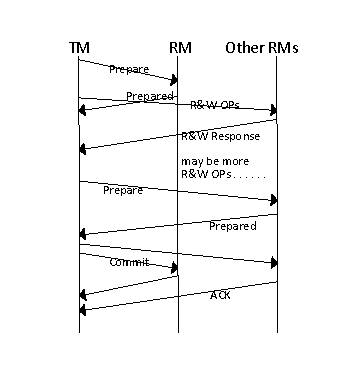
\includegraphics[scale=1] {transaction_oneshot}  \label{fig:transaction_NDP}  }
    \captionsetup[subfigure]{oneside,margin={0.25cm,0cm}}
    \subfloat[DP transaction, ${RM}$ would be told other ${RM}$'s state when receiving \emph{Prepare}]
        { 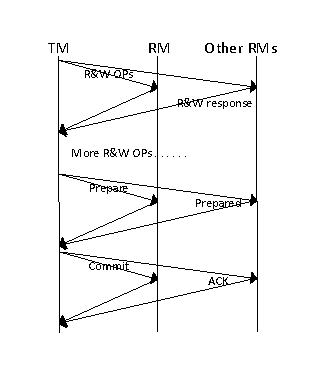
\includegraphics[scale=1]{transaction_interactive} \label{fig:transaction_DP}}

  \caption{Commit message flows for DP and NDP distributed transactions}
  \label{fig:transaction_type}
\end{figure}


\subsection{Scheduling of Distributed Transactions}
Before presenting the idea of lock violation, we first review the conceptual model of distributed transaction processing,
which has been formalized in previous work, such as \cite{LockNoWait:journals/csur/BernsteinG81}.

\subsubsection{Transaction and Schedule}
Suppose that a distributed database resides on ${n}$ nodes, represented by: 

  ${R = \{r_1, r_2, ... r_n\}}$.

A transaction ${T_i}$ runs on ${m}$ of the ${n}$ nodes ($1 \le m \le n$).%, represented by  ${S = \{s_1, s_2, ... s_m\} \subseteq R}$,
The transaction ${T_i}$ is composed of a series of operations,
each of which can be a read or a write or other command operation including abort, commit, etc.
Let ${r_i[x]}$ denote that ${T_i}$ reads the record ${x}$. Let ${w_i[x]}$ denote that ${T_i}$ writes on the record ${x}$.
Let ${c_i}$, ${a_i}$, ${p^c_i}$, ${p^a_i}$ denote the commit, abort, prepare-to-commit and prepare-to-abort operations of ${T_i}$ respectively.


A transaction schedule is a collection ${H = \{h_1, h_2, ..., h_n\}}$.
Each ${h_u}$ is the local schedule of $H$ on the node ${s_u}$, which is a sequential history of operations issued by different transactions.
%For instance, Fig. \ref{fig:strict_example} illustrates a transaction schedule over three nodes.

\subsubsection{Deterministic and Non-deterministic Abort}

Several reasons can cause a transaction to abort. In general, we categorize them as:

1. User requested abort.
These are aborts specified by the program logic (e.g., a transaction requires to abort if it has accessed a non-existent record).

2. System demanded abort.
These are aborts commanded by the database system.
There are several situations that the system will abort a transaction.
For instance, if OCC is applied, a transaction will be aborted in case of a potential violation of isolation.
If deadlock detection is applied to break a wait-for circle,
the scheduler would choose a transaction as a victim to abort.

3. Database node failure.
When a node fails, the system is forced to abort the transactions running on the node. For simplicity, we assume that there are fail-stop failures only.

We call the first two types of abort \emph{deterministic abort} and the last one \emph{non-deterministic abort}.
In a database system, deterministic aborts occur much more frequently than non-deterministic aborts.
Therefore, the prices we are willing to pay for the two kinds of abort are very different.

\subsubsection{Dependencies among Transaction}

There are three types of data dependency among transactions,
\emph{wr-dependency},
\emph{ww-dependency}
and \emph{rw-dependency}.

In a local schedule ${h}$, if ${T_j}$ reads ${T_i}$'s write on ${x}$,
we call it a \emph{read-after-write(wr) dependency} and denote it by ${w_i[x] \rightarrow r_j[x]}$.
Analogically, if ${T_j}$ overwrites ${T_i}$'s write on ${x}$, it is called a \emph{write-after-write(ww) dependency} and denoted by ${w_i[x] \rightarrow w_j[x]}$.
If ${T_i}$ reads ${x}$ before ${T_j}$ writes on ${x}$, it is called a \emph{write-after-read(rw) dependency} and denoted by ${r_i[x] \rightarrow w_j[x]}$.
Based on data dependencies, we can define \emph{commit dependency}. ${T_j}$ has a \emph{commit dependency} on ${T_i}$, written as ${T_i \rightarrow T_j}$, if ${T_j}$ cannot commit prior to ${T_i}$.
More detailed concepts of dependency can be found in \cite{Dependency:conf/sigmod/ChrysanthisR90} \cite{Dependency:conf/sigmod/BilirisDGJR94}
%cite{TODO}

\subsubsection{Relaxation on Correctness Criteria}

Traditional database systems adopt Strict Two-Phase Locking (S2PL) \cite{DBLP:conf/vldb/Raz92} to ensure serializability and recoverability.
Strictness implies that a transaction cannot read a previous write by another transaction that has not been committed yet.
Strictness is not a necessary condition for a correct schedule.
Although it simplifies the implementation of a database system, it sacrifices the concurrency of transaction processing.

%For instance, the schedule ${H_1}$ of Fig. \ref{fig:strict_example} is serializable and strict.
%(The data dependencies include ${r_1[x] \rightarrow w_3[x]}$, ${w_1[x] \rightarrow r_2[y]}$, ${r_2[y] \rightarrow w_3[x]}$, which are not cyclical.)
In contrast, ${H_1}$ in Fig. \ref{fig:non_strict_example} is serializable but not strict.
As we can see, there are three records ${x}$, ${y}$, ${z}$, residing on ${s_1}$, ${s_2}$, ${s_3}$ respectively.
${T_1}$ writes ${y}$ and ${x}$.
${T_2}$ reads ${T_1}$'s write on ${x}$ before ${T_1}$ commits.
Transaction ${T_3}$ overwrites ${T_2}$'s write before ${T_2}$ commits.
By violating strictness, ${H_1}$  enables a higher degree of concurrency.


\begin{figure}[tbp]
  \centerline{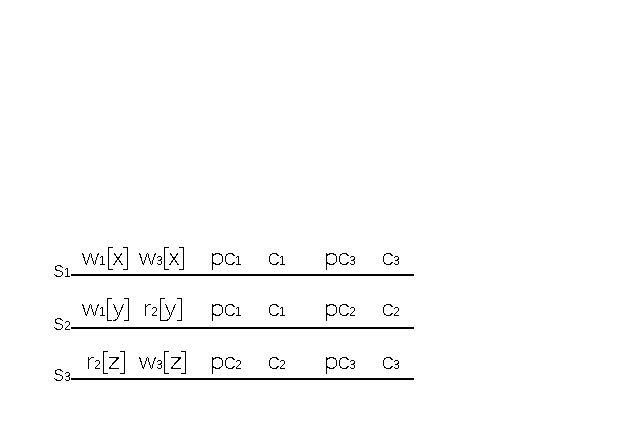
\includegraphics[scale=1]{schedule_non_strict.pdf}}
  \caption{A non-strict but serializabile schedule ${H_1}$}
  \label{fig:non_strict_example}
\end{figure}

\begin{figure}[tbp]
  \centerline{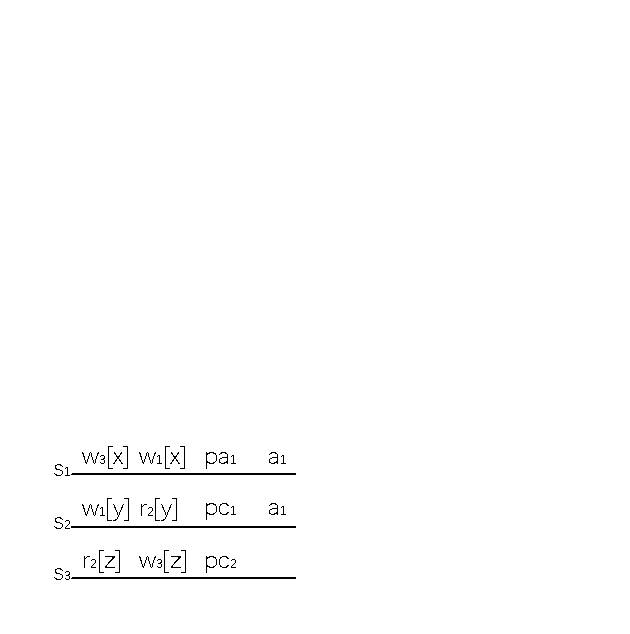
\includegraphics[scale=1]{schedule_not_serializabile.pdf}}
  \caption{Schedule ${H_2}$, ${T_1}$ abort due to non-serializabile}
  \label{fig:schedule_abort_example}
\end{figure}

\begin{figure}[tbp]
  \centerline{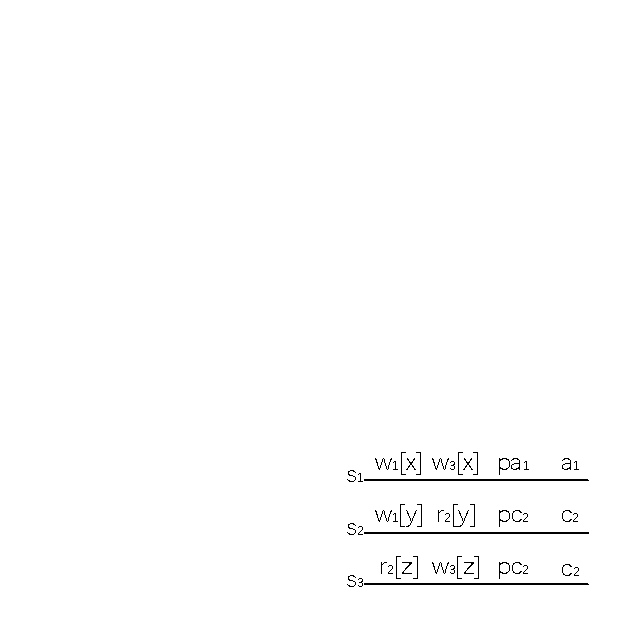
\includegraphics[scale=1]{schedule_not_recoverable.pdf}}
  \caption{Schedule ${H_3}$, ${T_2}$ commit ahead ${T_1}$, non-recoverable anomaly}
  \label{fig:schedule_not_recoverable}
\end{figure}


The drawback of strictness is further amplified by replication and commit protocols in a GDDB.
The commit of a transaction in a GDDB usually involves a lot of work, including multiple rounds of communication across the WAN.
As strictness requires a transaction to hold locks until it finishes committing, this means a substantially lengthened locks' blocking time.
Lengthened lock blocking time can severely hurt the performance of distributed transactions.
Therefore, we are inclined to embrace a non-strict scheduler.

Relaxation on strictness will, however, complicate the recovery mechanism.
In a traditional recovery mechanism, such as ARIES\cite{ARIES:journals/tods/MohanHLPS92}, the transactions' dependencies completely comply with their logs' persisting order.
Log order guarantees the recoverability of scheduling, which requires that a transaction not commit before the transactions depend on (in terms of commit dependency).
When strictness no longer holds, we need other tactics to enforce recoverability, which may incur additional overheads.
When both serializability and recoverability (not necessarily strictness) are ensured, we regard the schedule as a correct schedule.


\subsection{Lock Violation and Dependency Tracing}

Lock violation is a general technique to enable a non-strict scheduler.
Its basic idea is to allow a transaction to speculatively access data locked by other transactions.
If such speculative data accesses cause a problem, the system uses a mechanism to rectify it.

For lock violation to be correct, it should first preserve serializability.
Considering the schedule ${H_2}$ in Fig. \ref{fig:schedule_abort_example},
it contains three data dependencies:

\begin{center}
${w_3[x] \rightarrow w_1[x]}$,
${w_1[y] \rightarrow r_2[y]}$
${r_2[z] \rightarrow w_3[z]}$
\end{center}

This leads to a circle ${T_1 \rightarrow T_2 \rightarrow T_3 \rightarrow T_1}$, which makes the schedule non-serializable.
${H_2}$ is not possible if we apply S2PL.
It becomes possible when lock violation is permitted -- we allow ${T_2}$ to read from uncommitted ${T_1}$, and ${T_1}$ to overwrite uncommitted ${T_3}$.
Therefore, to preserve serializability, we need to prevent the data dependencies from forming a dependency cycle.
Many techniques can be adopted to achieve this, including the \emph{wait-die} strategy mentioned in the related work.

A schedule generated by lock violation must also be recoverable.
In the schedule ${H_3}$ in Fig.   \ref{fig:schedule_not_recoverable}, due to lock violation,
${T_2}$ reads  ${T_1}$'s write and commits before ${T_1}$.
In this case, if ${T_1}$ decides to abort later, it is no longer possible to revert ${T_2}$.
Therefore, ${H_3}$ is not a recoverable schedule.
To ensure recoverability, we need to trace the commit dependencies among transactions and force the commit order to comply with the commit dependencies.
If we know that ${T_2}$ depends on ${T_1}$, we can hold ${T_2}$'s commit request until ${T_1}$ finishes.
If ${T_1}$ decides to abort, we abort ${T_2}$ too.
This behavior is known as \emph{cascade abort}.
Cascade abort can be caused by a deterministic abort or a non-deterministic abort.

In summary, dependencies among transactions need to be somehow traced when lock violation is in use to ensure serializability and recoverability.

\section{Design of DLV}
\label{sec:implement}

In this section, we present our design of Distributed Lock Violation (DLV).

\subsection {Timing of Lock Violation}


In a distributed transaction, $TM$ assigns work to $RM$. Once the work is done, $TM$ applies 2PC to end the transaction.
In 2PC, both $TM$ and $RM$ need to synchronize with their replicas to make sure that node failures will not corrupt the data.
Synchronization usually takes a long time, especially when the replicas are remotely located.
DLV aims to shorten the lock blocking time through lock violation.
In a GDDB, lock blocking time can be significantly shortened if we violate locks before data synchronization starts.

We classify lock violation into two types, early lock violation (or early violation for short) and late lock violation (or late violation for short).
In early violation,  we allow a transaction's locks to be violated before its serial order can be determined.
In late violation,  we allow a transaction's locks to be violated after its serial order is determined.

More specifically, when the two-phase commit is adopted, there are several occasions to perform lock violation.
We classify the timing of lock violation into four categories:

\emph{DLV0}:
Once a transaction finishes a read operation or a write operation, other transactions can immediately violate the lock.
In other words, a transaction can violate a lock at any time.
In this case, serializability needs to be ensured by dependency tracing but not locking.

\emph{DLV1}:
After an ${RM}$ of a distributed transaction finishes its data processing operations on the local node, but before it persists its `prepare commit' state, other transactions can violate this transaction's lock.
Although locking can ensure a local schedule's serializability, it cannot guarantee the global serializability because some ${RM}$s may perform deterministic abort.
NDP transactions are in this case.

\emph{DLV2}:
When a transaction has entered the second phase of 2PC and received the decision made by the ${TM}$ to commit the transaction, it allows other transactions to violate its locks.
In this case, global serializability can be ensured by locking. Therefore, lock violation does not need to worry about serializability.

\emph{DLV1x}:
DLV1x is an optimized method for DLV1.
Before lock violation is enabled, ${TM}$ performs a serializability test, in which it communicates with all ${RM}$.
If all ${RM}$ agree to commit, the test will be passed, and lock violation will be enabled.
In this case, global serializability can be guaranteed too. And it can perform lock violation earlier than DLV2.
However, this may require an additional message round trip for an NDP transaction.
Fortunately, this message round trip can overlap with the 2PC and replication message flows.
In a GDDB in gathered leader mode(replicas leader are enforced in the same AZ), as this message round trip does not occur between geo-replicated nodes, it is not expensive.
%\begin{highlighted}
DLV1x adds a serializability test message round trip to the 2PC message flow.
In this round trip, a \emph{RM} responds \emph{Violate Vote Yes} if it has executed all its access successfully.
This message promise that the \emph{RM}: 1. It will not run any more access actions; 2. if it adds all its access action into the local history, there is no serializability violation.
\emph{TM} collects \emph{RM}'s \emph{Violate Vote Yes} messages and send \emph{Violate Enable} message to notify \emph{RMs} makes their locks be violative.
We can technically merge this message round trip with other data access or 2PC messages to save cost.
As a result, DLV1x and DLV1 become the same thing for DP transactions.

\begin{figure}[tbp]
  \centerline{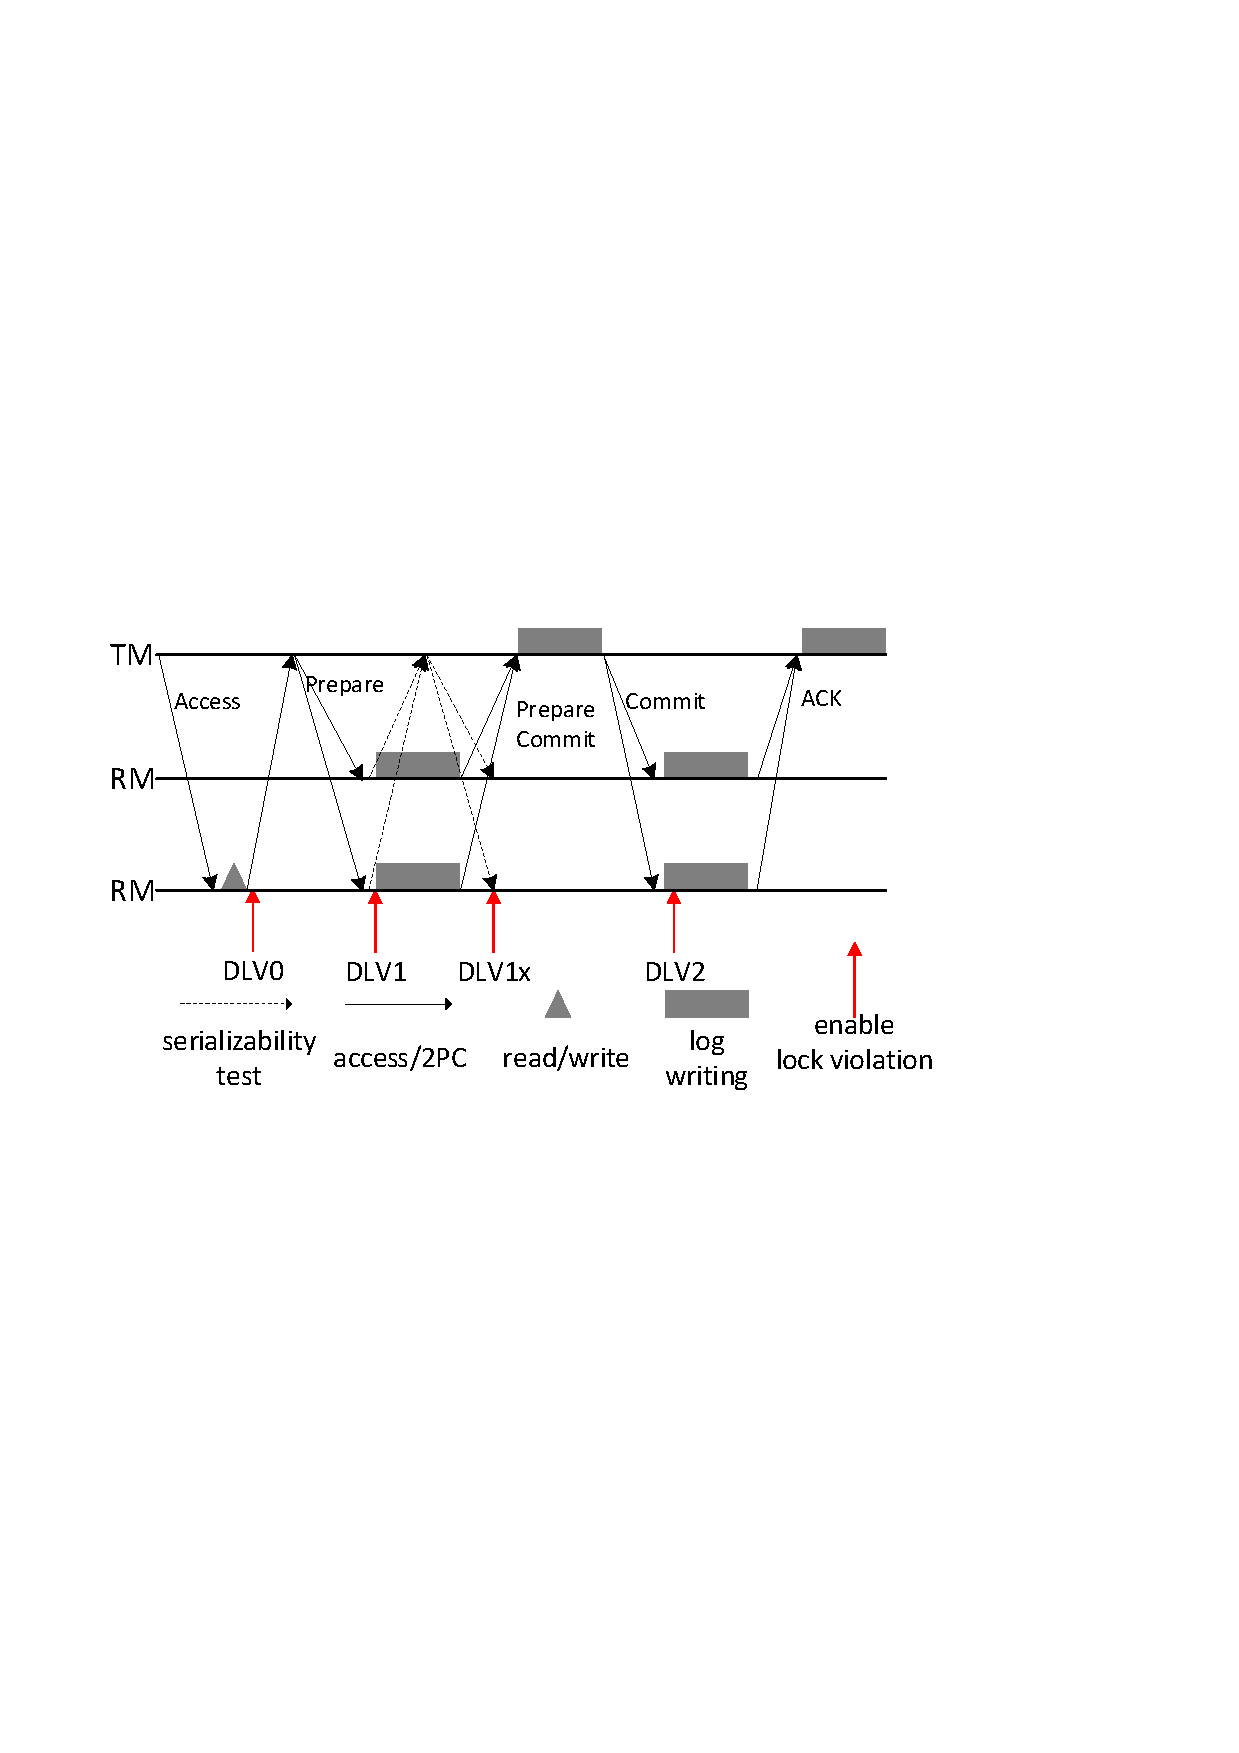
\includegraphics[scale=0.50]{lock_violation_time.pdf}}
  \caption
  {Timing of enabling lock violation}
\label{fig:lock_violation_time}
\end{figure}

Fig.~\ref{fig:lock_violation_time} illustrates the different timings of lock violation.

We can infer that DLV0 and DLV1(for NDP transaction) are early violation, and DLV1x and DLV2 are late violation.
Early violation allows us to violate lock earlier so we can harness more concurrency. However, there are a few prices it needs to pay.

First, when the early violation is performed, we can no longer rely on locking to ensure serializability. This has been illustrated by ${H_2}$ in Fig.~\ref{fig:schedule_abort_example}.
Therefore, the early violation has to resort to other measures, such as data dependency tracing, to ensure serializability.
In contrast, the late violation is safe on serializability.
We define a transaction's \emph{safe violation time} as the time interval in which its locks can be violated without breaking serializability.
As illustrated by Fig. \ref{fig:lock_violation_safe},
There is no safe violation time for the early violation, as there is no way to determine when lock violation can be safe unless it performs a serializability test as DLV1x does.


Second, the early violation may face a much higher abort rate due to an increased chance of serializability violation and cascade abort.
In late lock violation, only non-deterministic aborts can cause cascade abort, as no lock can be violated before a deterministic abort.
In early lock violation, all types of aborts can cause cascade abort.

Third, if early violation relies on dependency tracing to ensure serializability, it will incur more overheads.
Whether early or late violation is adopted, we need to trace the commit dependencies among transactions to ensure the commit order (or recoverability).
However, early violation needs to trace all \emph{rw, ww, wr} dependencies, while late violation only needs to trace \emph{wr} dependencies.

%\end{highlighted}

\begin{figure}[tbp]
  \centerline{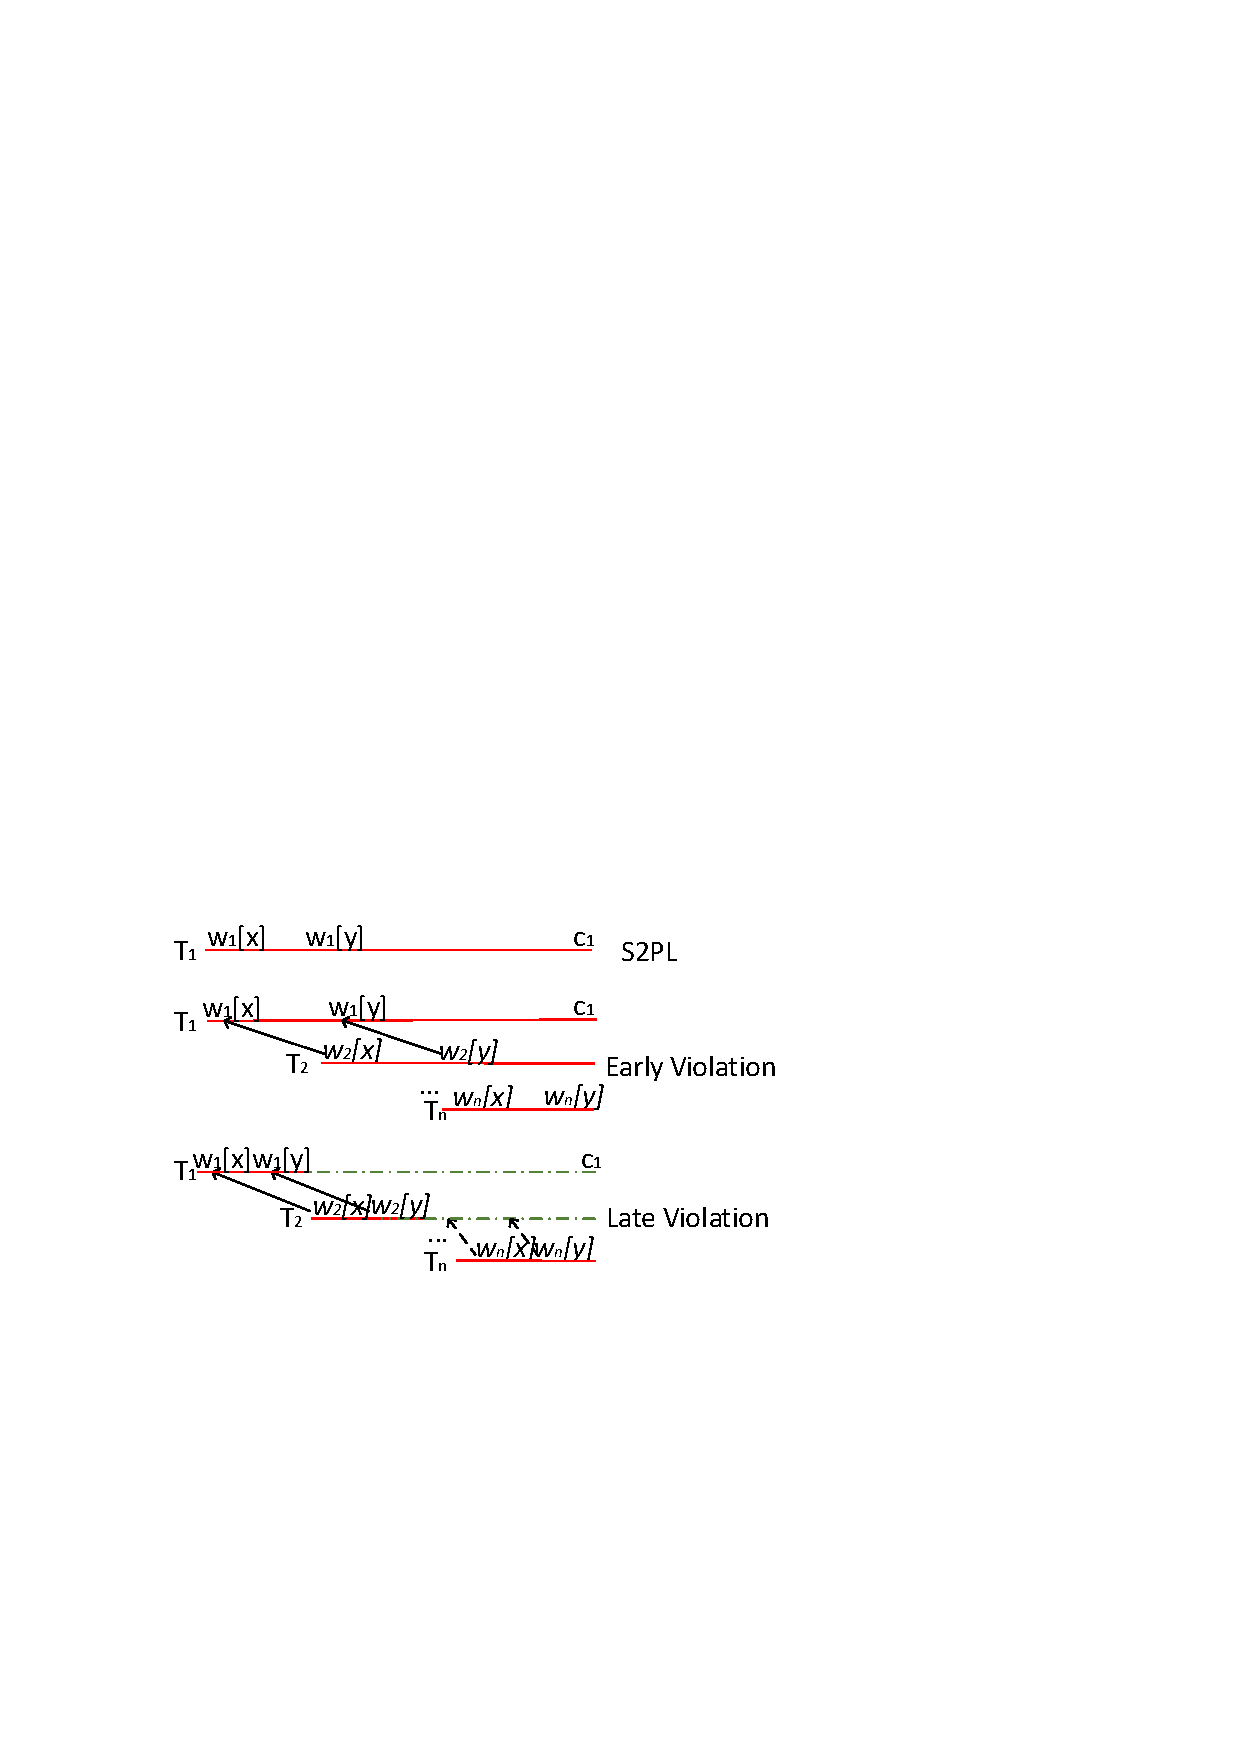
\includegraphics[scale=0.6]{lock_violation_safe.pdf}}
  \caption
  {The green dash line shows the safe violation time of late violation.
  Early lock violation has no safe violation time.
  The italicized text shows the operation after lock violation actions}
\label{fig:lock_violation_safe}
\end{figure}

\subsection{Dependency Tracing}
As discussed previously, when lock violation is in use,
the scheduler must trace commit dependencies to ensure recoverability.
If early lock violation is adopted, the scheduler needs to trace more dependencies (including all \emph{rw, wr, ww}-dependencies) to ensure serializability.
(For late lock violation, we only need to ensure recoverability.
It will be enough to trace \emph{wr} dependencies only.)

DLV applies the register-and-report method~\cite{HeckatonMVCC:journals/pvldb/LarsonBDFPZ11} to trace commit dependencies.
Each transaction maintains an in-dependency count ${in}$ on each of its ${RM}$s, which records the number of transactions it depends on that ${RM}$.
Each transaction also maintains an out-dependency set  ${out}$ on each of its ${RM}$s, which records all the transactions depending on it on that ${RM}$.
When a transaction ${T}$ violates another transaction ${S}$'s lock on a ${RM}$,
DLV would register the commit dependency by adding ${T}$ to the corresponding ${out}$ set of ${S}$ and incrementing the corresponding ${in}$ of ${T}$ by one.
A ${RM}$ will not vote to commit (or prepare commit) if its ${in}$ dependency count is greater than 0, suggesting that the DB has not yet committed some of its in-dependency transactions.
When a transaction aborts, it notifies all its out-dependency transactions to abort (cascade abort) by setting their ${in}$ dependency counts to a negative value.
(If a transaction finds that one of its ${in}$ dependency counts is negative, it will abort automatically.)
When a transaction commits, it will traverse its ${out}$ sets and decrease the corresponding ${in}$ value of each transaction in the ${out}$ set by one.
%\begin{highlighted}

Note that each $RM$ node independently maintains the dependency information locally.
We do not allow a ${RM}$ to enter an undecidable state (e.g., the `prepare commit' state) before its in-dependency count ${in}$ becomes zero.

If a transaction's ${in}$ value on a ${RM}$ is greater than 0, it implies that not all the transactions it depends on have committed.
We can then guarantee that this ${RM}$ will not enter the uncertain ``prepare commit'' state.

When a node fails, all the un-prepared ${RM}$s on the node can vote to rollback their transactions without referring to the dependency information.
In this case, both the ${in}$ values and the ${out}$ sets on the node become useless.
Therefore, the system only needs to preserve the dependency information in memory without persisting it to stable storage.

%\end{highlighted}
\subsection{Cascade Abort Handling}
When a cascade abort occurs,
we need to undo a number of transactions.
(When late lock violation is in use, cascade abort can only be triggered by a node failure.)
In case of failure, traditional DB systems use undo logs to cancel out a transaction's write operations.
Undo becomes a bit tricky in DLV.

For a centralized DB, its scheduler can utilize the chronological order of the logs to perform undo.
During system recovery, the database can play the undo logs in reverse order, just as what ARIES does.
For a distributed DB, a global undo order cannot be easily achieved.

If undo is performed locally by each transaction, it may produce anomalies.
Consider the following example. Suppose two tuples $x$ and $y$ are located at two nodes.
Two distributed transactions $T_1$ and $T_2$ access both $x$ and $y$, and result in a global schedule:

\begin{center}
${H_4 = ...w_1[x]w_1[y]r_2[x]w_2[y]a_1a_2}$
\end{center}

When a node fails, ${T_1}$ aborts, which forces ${T_2}$ to abort too.
The aborts trigger undo operations, which extend ${H_4}$ to ${exp(H_4)}$,
in which ${w^-_i[x]}$ denotes that ${T_i}$ undoes its write on ${x}$.

\begin{center}
  ${exp(H_4) =  w_1[x]w_1[y]r_2[x] w_2[y]}$
  ${w^-_1[x]w^-_1[y]  c_1 w^-_2[y]c_2}$
\end{center}


\begin{table}[tbp]
  \centering
  \caption{local schdeule $h_1$ and $h_2$, $x$ and $y$'s values, undo log after the execution of ${exp(H_4)}$}
  \begin{tabular}{|c|c|c|c|c|c|c|c|}
  \hline
steps & $h_1$ & $x$ & $h_2$ & $y$ & undo   \\
  \hline
  \hline
 1& $w_1[x=1]$ & 1 & &  0 & x=0  \\
  \hline
  2& & 1 & $w_1[y=1]$ & 1 & y=0   \\
  \hline
3 & $r_2[x]$ & 1 & & 1 &    \\

  \hline
 4 & failure  & 1 & & 1 &  \\
  \hline
 5& & 1 &   $w_2[y=2]$ & 2 & y=1  \\
  \hline
6  & $w^-_1[x=0]$ & 0 && 2 &   \\
  \hline
7 & & 0 & $w^-_1[y=0]$ & 0 &   \\
  \hline


8  & $c_1$ & 0 &$c_1$& 0 &   \\
  \hline
9 & & 0 &  $w^-_2[y=1]$& 1 &   \\
  \hline
10 & $c_2$ & 0 &$c_2$& 1 &  \\
  \hline
  \end{tabular}

\label{tbl:x_y_vlues}
\end{table}

In $exp(H_4)$, the two transactions perform undo independently. $exp(H_4)$ results in an anomaly.
Table~\ref{tbl:x_y_vlues} shows the local schedules of $exp(H_4)$, i.e., ${h_1}$ and  ${h_2}$, and how ${x}$ and ${y}$ change as we carry out the operations.
(Suppose the initial values of ${x}$ and ${y}$ are both 0.)
In step 4, the node hosting ${x}$ fails and restarts.
As we can see, after both ${T_1}$ and ${T_2}$ abort, the value of ${y}$ becomes 1, which is incorrect.

To ensure correctness, we have to follow the reverse order of the write operations to perform undo.
For ${H_4}$, a correct undo schedule should be:
\begin{center}
${exp^*(H_4) = w_1[x]w_1[y]r_2[x]w_2[y]w^-_2[y]c_2w^-_1[y]w^-_1[x]c_1}$
\end{center}

To tackle this problem, we need a complex algorithm, such as SOT \cite{UnifyCR:journals/is/AlonsoVABASW94}.
To reduce complexity, DLV adopts the no-steal policy in logging.
The no-steal policy forbids the system from writing uncommitted data to permanent storages.
As a drawback, it may consume more memory space.
Considering that today's database servers usually have large RAM, this is no longer a big concern.
Based on this design, we need no undo logs anymore. If a transaction aborts, we only need to discard its uncommitted data in memory.
The no-steal policy has another advantage in GDDB.
Using No-steal, a transaction can push the work of data synchronization to the commit phase.
Thus, through lock violation, we can exclude data synchronization completely from the lock blocking duration.

When multiple concurrent transactions modify the same data, this data can have multiple versions in memory.
Therefore, DLV needs to maintain a version list for each data item.
There is only one version for each data item in the permanent storage, the newest committed version.
Using multiple versions and no-steal, the old data can be restored easily.
Another side benefit of getting multiple versions is fewer dependencies maintaining cost for late violation.
Fig.~\ref{fig:versions_example} illustrates why cascade abort only need to consider $wr$ dependencies but not $ww$ dependencies for late violation. 
Suppose a number of transactions accessed two tuples, ${x}$ and ${y}$.
The green rectangles represent the uncommitted versions of the version lists' data, and the red ones represent the committed versions.
We can see that although there is a ${ww}$ dependency ${w_6[x] \rightarrow w_4[x]}$,
the abort of $T_4$ does not require ${T_6}$ to abort.
\begin{figure}[tbp]
  \centering
  \captionsetup[subfigure]{margin={0cm,0cm}}
  \subfloat[${H_a}$]
  {
    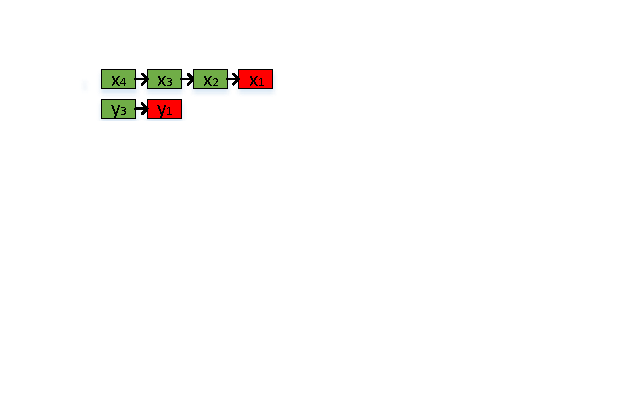
\includegraphics[scale=1.2] {version1} \label{fig:versions_a}}
    \captionsetup[subfigure]{margin={0cm,0cm}
  }
  \subfloat[\small ${H_b}$]
  {
    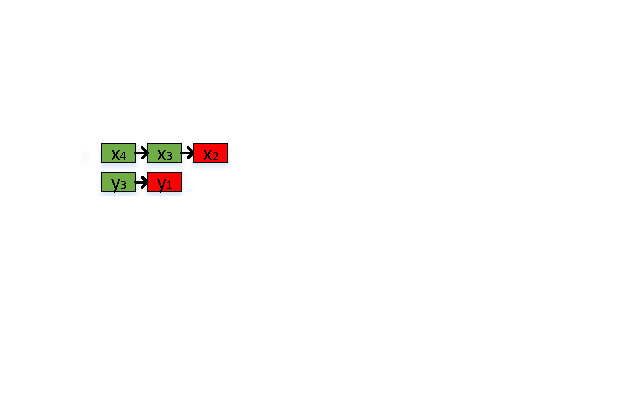
\includegraphics[scale=1.2]{version2} \label{fig:versions_b}
  }
    \captionsetup[subfigure]{margin={0cm,0cm}
  }
  \subfloat[\small ${H_c}$]
  {
    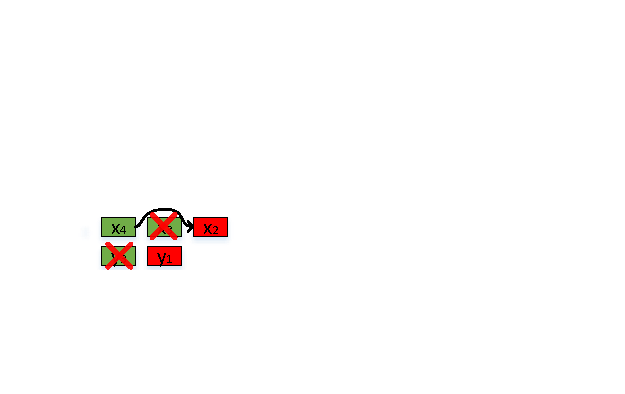
\includegraphics[scale=1.2] {version3} \label{fig:versions_c}}
    \captionsetup[subfigure]{margin={0cm,0cm}}
    \subfloat[\small ${H_d}$]
      { 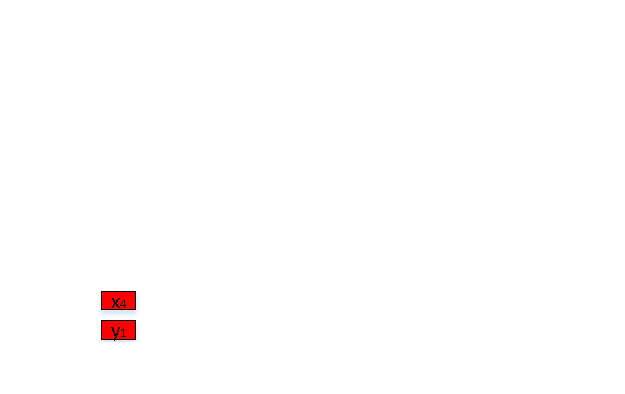
\includegraphics[scale=1.2]{version4} \label{fig:versions_d}
  }
  \caption{\emph{ww}-dependencies are not required for recovery.
  ${x_i}$ represents the version of $x$ created by ${T_i}$.
 Then, $w_j[x_i]$ represents that ${T_j}$ overwrites the write of ${T_i}$ on $x$. In the history, ${H_a = w_1[x_0]w_1[y_0]c_1w_2[x_1]w_3[x_2]w_3[y_1]w_4[x_3]}$, 
 ${H_b = H_a c_2r_5[y_3]w_6[x_4]}$,
 ${H_c = H_b a_3a_5}$, 
 ${H_d = H_c c_4r_6[y_1]c_6}$
}
\label{fig:versions_example}
\end{figure}


\subsection {Deadlock Handling}
\label{sec:deadlock_handling}
When we apply lock violation, deadlock can occur.
There are various approaches to handle deadlock.
Deadlock detection is the most widely used approach in a centralized DB.
Deadlock detection needs to maintain a waits-for graph (WFG).
In a distributed environment, maintaining a WFG is expensive.


Another approach to handling deadlock is deadlock prevention, which is simpler but more restrictive.
Different deadlock handling techniques may suit different lock violation methods.
For instance, the early violation may work better with deadlock detection, while late violation may work better with deadlock prevention.

Out implementation of deadlock prevention uses the \emph{wait-die} protocol to prevent deadlocks and preserve serializability.
A transaction is assigned a unique timestamp when it starts.
(This does not require a centralized timestamp allocator.
Each node can generate a unique timestamp for its transactions by combining its local clock time and node id.)
Then, conflicting transactions can be ordered by their timestamps.
Following the \emph{wait-die} protocol, a transaction will wait if it attempts to access a data item locked by a transaction with a larger timestamp.
It will abort if the data item is locked by a transaction with a smaller timestamp.
Only allowing a transaction to violate a lock with a larger transaction id can guarantee that the data dependencies are acyclic.


Early lock violation may suffer a higher abort rate if we adopt lock prevention.
Given a set of transactions ${T_1, T_2... T_n}$, their IDs follows a total order, ${T_1 < T_2 < ... < T_n}$.
Their dependencies are in the form ${T_1 \rightarrow T_2 ... \rightarrow T_n}$.
In \emph{wait-die}, ${T_2, ..., T_n}$ must abort due to lock violation's \emph{wait-die} policy(a larger transaction id must abort when encountered conflict lock of a smaller transaction id) even there is no serializability violation.

In the same time window from transaction ${T_1}$'s start to its end, only transaction ${T_1}$ can commit.
In this case, the violation scheduler performance is the same as the S2PL scheduler.
If the scheduler took the deadlock detection approach, transaction ${T_2, ... T_n}$ would not necessarily abort because there was no deadlock.
Early lock violation performance using deadlock detection for this case may be better than deadlock prevention ones.
In the late lock violation case, dependency ${T_1 \rightarrow T_2 , ... ,T_n}$ would not contribute to non-serializability.
These dependencies are not necessarily traced by deadlock detection or be test by the \emph{wait-die} policy.
This late violation case can get better performance since ${T_2,..., T_n}$ can commit if there is no system failure.

\section{Experiments}
\label{sec:experiment}
We developed a GDDB engine to evaluate the performance of \emph{DLV}.
We conducted extensive experiments to compare different types of \emph{DLV} (DLV0, DLV1, DLV2, and DLV1x) against the traditional S2PL approach.
The goal was to understand how good \emph{DLV} is and what implementation of \emph{DLV} can yield the best performance. 

\subsection{Experimental Setting}
\label{subsec:exp_setting}

Our experiments were conducted in Ali-Cloud.
In total, 12 servers were used.
Each server was equipped with 12 virtual CPU cores of 2.5GHz and a 48GiB RAM.
The OS was Ubuntu 18.04.
The database partitioned its data into four shards.
Each shard had three replicas spread across three AZs,
located in Heyuan (South China), Hangzhou (East China), and Zhangjiakou (North China), respectively.
Every AZ had a full copy of each shard of data.
The internal network bandwidth in each AZ was 1Gbps.
We used another server as the client node dedicated to issuing transaction requests.
We used customized TPC-C and YCSB benchmarks to perform the evaluation.


TPC-C~\cite{TPCC:conf/tpctc/NambiarWMTLCM11} models a real-world scenario in which a company sells products through multiple warehouses in different districts, and customers order products and pay bills.
In our version of TPC-C, we partitioned the data mainly by the warehouse IDs.
The item table was not partitioned but replicated across all the shards.
Such a DB design enabled us to achieve the best performance.
As our purpose was to evaluate the performance of distributed transactions,
we made all the transactions distributed by enforcing each transaction to order items from warehouses located at different nodes.
We excluded the think time of TPC-C and only measured the performance of the NewOrder transactions.


YCSB~\cite{YCSB:conf/cloud/CooperSTRS10} was originally designed to evaluate NoSQL databases.
Its transactions are relatively simple.
Each YCSB transaction accesses nearly ten rows of data, which follow a Zipfian distribution.
By adjusting the Zipfian skewness (i.e., the parameter \emph{theta}), we can customize the degree of contention.
We partitioned the YCSB data by the primary key of the main table.
To make all transactions distributed, we forced each transaction to access at least two shards.

We evaluate the performance by TPM(the number of transactions committed in each minute).


\subsection{Deadlock Detection vs Deadlock Prevention}

To handle deadlock, DLV faces two options, deadlock detection or deadlock prevention, as discussed in Section~\ref{sec:deadlock_handling}.
It is not obvious which approach works better for DLV. 
Therefore, our first set of experiments was to compare the two approaches for handling deadlocks.
We implemented \emph{wait-die} as the deadlock prevention approach.
When the \emph{wait-die} policy is employed, blocking will be rare, and aborts will be the main obstacle to performance.
For deadlock detection, we implemented a de-centralized path-pushing deadlock detector\cite{Deadlock:journals/computer/Singhal89}.

We applied deadlock detection and deadlock prevention to all the DLV variants as well as S2PL. 
We evaluated these approaches using YCSB.
We increased the number of user terminals until the throughput of the database reaches its maximum.
The results of the experiments are shown in Fig.~\ref{fig:ycsb_deadlock} 


\begin{figure}[tbp]
  \centering
  \captionsetup[subfigure]{margin={0cm,0cm}}
  \subfloat[YCSB TPM]
      { 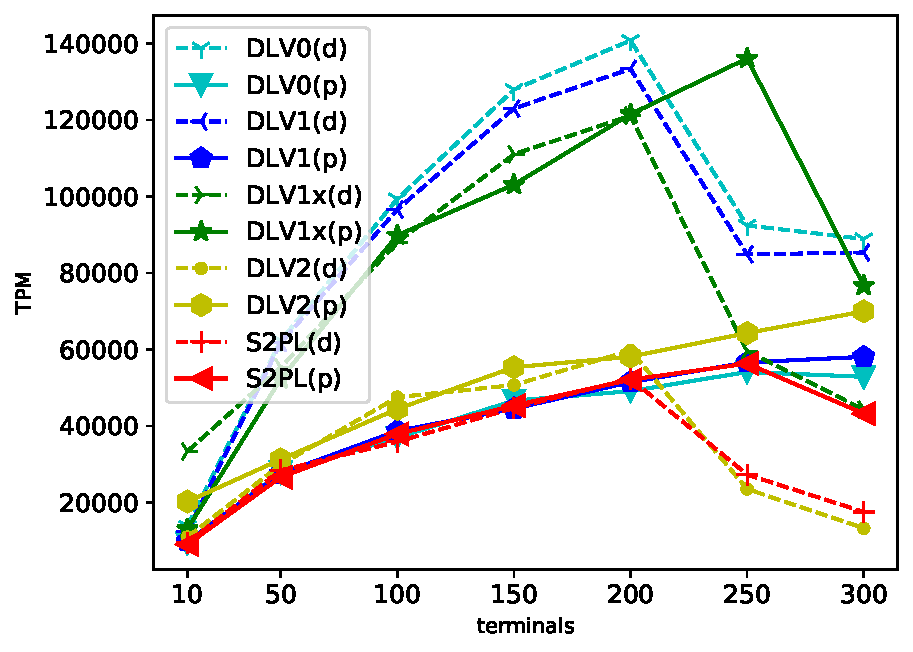
\includegraphics[scale=0.25] {plot_ycsb_terminal_g_o_tpm} \label{fig:ycsb_add_terminal_gathered:tpm}
      
      \captionsetup[subfigure]{margin={0cm,0cm}}
      
      }
      \subfloat[YCSB abort rate]
      { 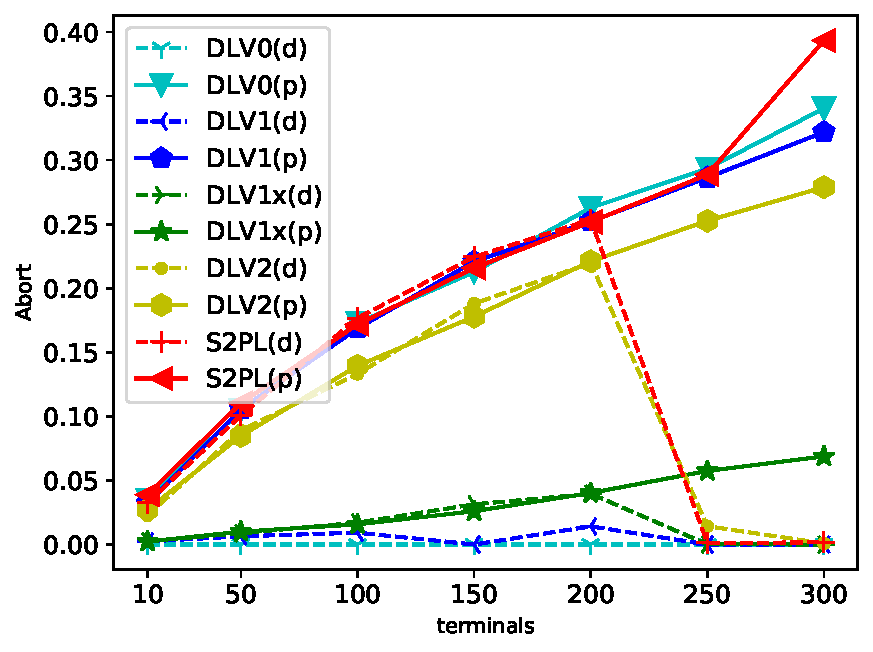
\includegraphics[scale=0.25]{plot_ycsb_terminal_g_o_abort} \label{fig:ycsb_add_terminal_gathered:abort}
      \captionsetup[subfigure]{margin={0cm,0cm}}
      }
      \caption{YCSB performance when increasing terminal numbers, including deadlock detection and deadlock prevention approach.
      ($(d)$ indicates adoption of deadlock detection. $(p)$ indicates adoption of deadlock prevention. ) }
      \label{fig:ycsb_deadlock}

\end{figure}

      
As we can see, there was no dominant winner. It is quite clear that deadlock detection works better for early lock violation, i.e., DLV0 and DLV1, 
and deadlock prevention works better for late lock violation, i.e., DLV1x and DLV2. This result is consistent with our analysis in Section~\ref{sec:deadlock_handling}.
Deadlock detection can be expensive when there is a high degree of contention. In contrast, deadlock prevention will incur a high abort rate to early lock violation.
We can see that if deadlock prevention is used, DLV0 and DLV1 cannot even outperform S2PL. 
%\begin{highlighted}
Deadlock detection does not scale well when the system is saturated.
As we can see, early lock violation could not scale to more than 200 terminals, but late lock violation could.
%\end{highlighted}
Nevertheless, a number of the DLV variants can outperform S2PL significantly. This means that lock violation can improve the performance of a GDDB.

Based on these results, in the rest of the evaluation, we applied deadlock detection to DLV0 and DLV1, and deadlock prevention to DLV1, DLV2, and S2PL, respectively,
as such configuration can maximize the performance of all the competing approaches.


\subsection{Impact of Geo-replication}

In the second set of experiments, we evaluated how geo-replication affects the performance of transaction processing.
We simulated geo-replication in a single AZ.
Namely, we put all replicas in the same AZ and artificially increased the replicas' communication latency.
We used the YCSB workload, in which we set the size of the data to 40,000 rows and the skewness (theta) to 0.2.
Fig.~\ref{fig:new_order_add_log_cost} shows how the throughput and the abort rate changed with the increased replication latency.
Geo-replication has a great impact on performance. The higher the replication latency, the lower the throughput of transaction processing.

We can also see that the DLVs performed significantly better than traditional S2PL in the experiments.
DLV0, DLV1, and DLV1x outperformed S2PL by 2-3 times when the replication latency is high.
While DLV2 slightly outperformed S2PL, too. It was inferior to other DLVs.
Because DLV2 does not violate locks early enough, and its lock duration overlaps with data synchronization among geo-replicas.
DLV1, DLV2, and S2PL adopted the \emph{wait-die} protocol; transactions were chosen to abort when confronted with serious contention.
Therefore, the abort rates measure how the performance was affected by contention.
The result shows that DLV1x could deal with contention better than DLV2 and S2PL.

\begin{figure}[tbp]
  \centering
  \captionsetup[subfigure]{margin={0cm,0cm}}
  \subfloat[YCSB TPM]
      { 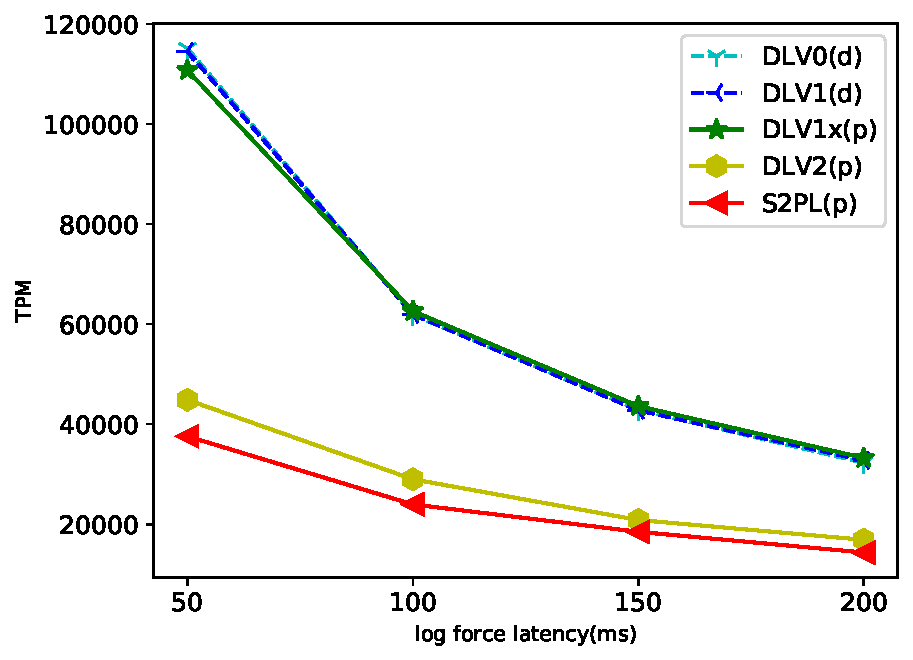
\includegraphics[scale=0.25] {plot_ycsb_latency_g_o_tpm} \label{fig:new_order_add_log_cost:tpm}
      
      \captionsetup[subfigure]{margin={0cm,0cm}}
      
      }
      \subfloat[YCSB abort rate]
      { 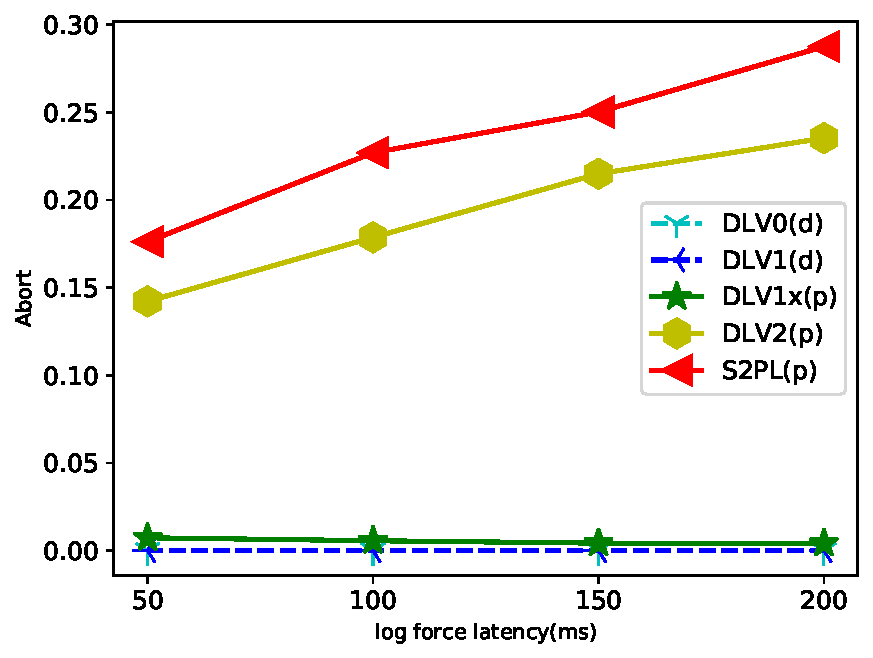
\includegraphics[scale=0.25]{plot_ycsb_latency_g_o_abort} \label{fig:new_order_add_log_cost:abort}
      \captionsetup[subfigure]{margin={0cm,0cm}}
      }
      \caption{Impact of Geo-distance(YCSB) }
      \label{fig:new_order_add_log_cost}
\end{figure}




\subsection{Impact of Contention}

Our third set of experiments aimed to evaluate how the degree of contention affects transaction processing performance.
We used both the TPC-C workload and the YCSB workload.
We ran all the experiments in a real geo-replication environment described in Section~\ref{subsec:exp_setting}.
We adopted the gathered mode in the experiments, which assumes that all replica leaders co-locate in the same AZ.


\begin{figure}[tbp]
  \centering
  \captionsetup[subfigure]{margin={0cm,0cm}}
  \subfloat[NewOrder TPM]
      { 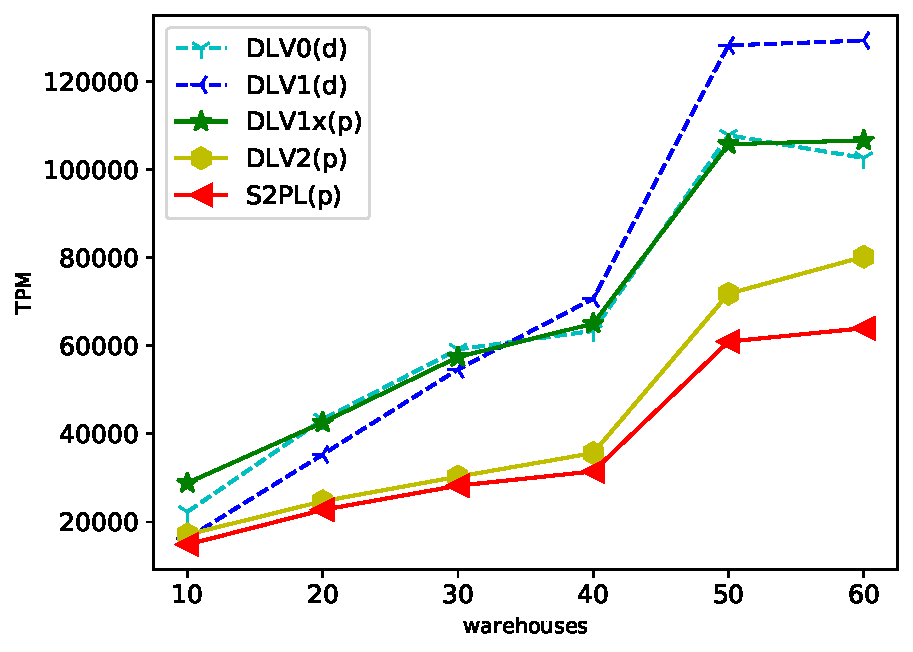
\includegraphics[scale=0.25] {plot_tpcc_warehouse_g_o_tpm} \label{fig:plot_tpcc_neworder_add_Warehouse_Warehouse_gather:tpm}
      
      \captionsetup[subfigure]{margin={0cm,0cm}}
      
      }
      \subfloat[NewOrder abort rate]
      { 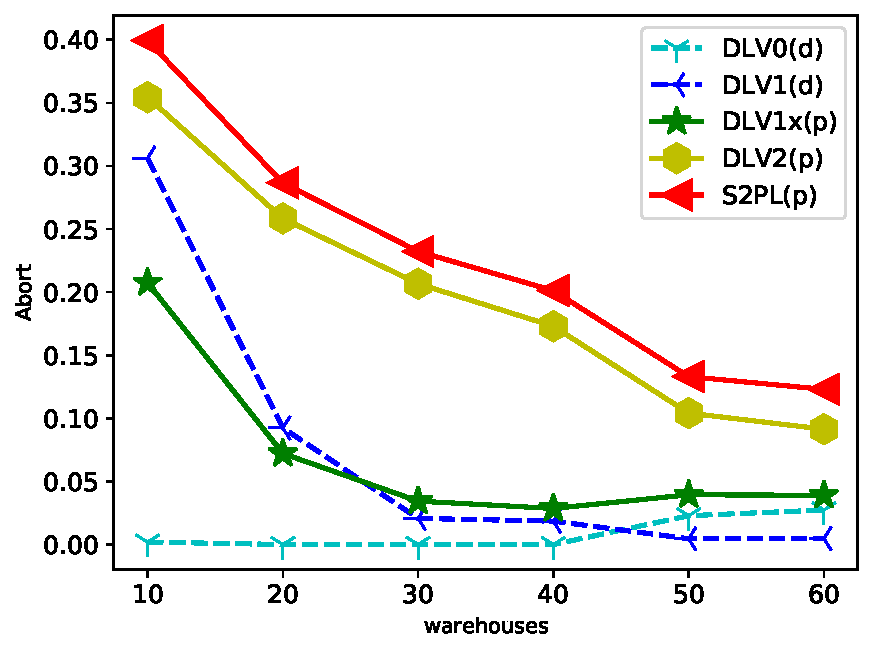
\includegraphics[scale=0.25]{plot_tpcc_warehouse_g_o_abort} \label{fig:plot_tpcc_neworder_add_Warehouse_Warehouse_gather:abort}
      \captionsetup[subfigure]{margin={0cm,0cm}}
      }
      \caption{Impact of Warehouse number(TPC-C) }
      \label{fig:plot_tpcc_neworder_add_Warehouse_Warehouse_gather}
\end{figure}




\begin{figure}[tbp]
  \centering
  \captionsetup[subfigure]{margin={0cm,0cm}}
  \subfloat[NewOrder TPM]
      { 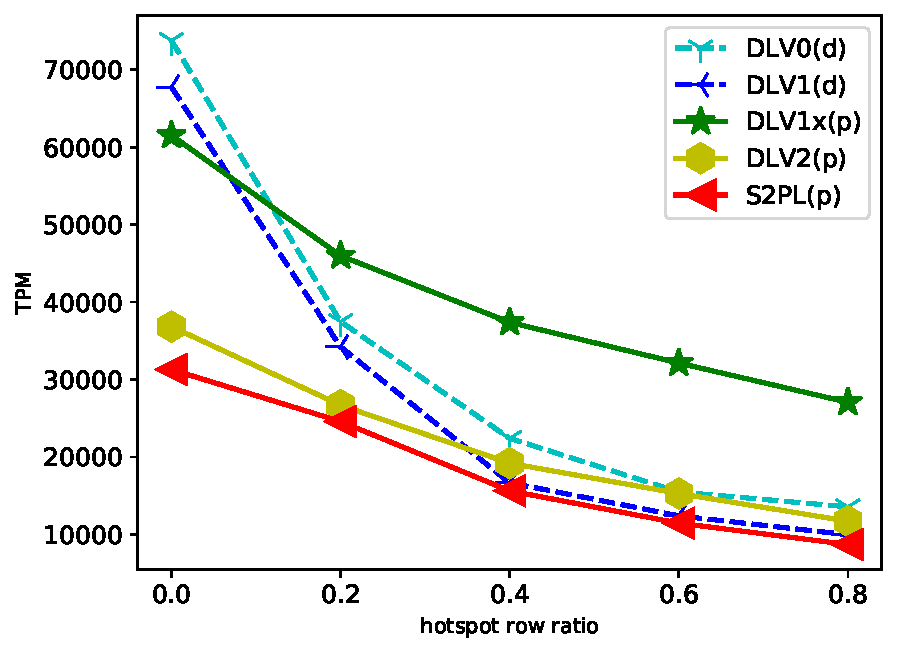
\includegraphics[scale=0.25] {plot_tpcc_hotitem_g_o_tpm} \label{fig:plot_tpcc_neworder_add_HotItem_HotItem_gather:tpm}
      
      \captionsetup[subfigure]{margin={0cm,0cm}}
      
      }
      \subfloat[NewOrder abort rate]
      { 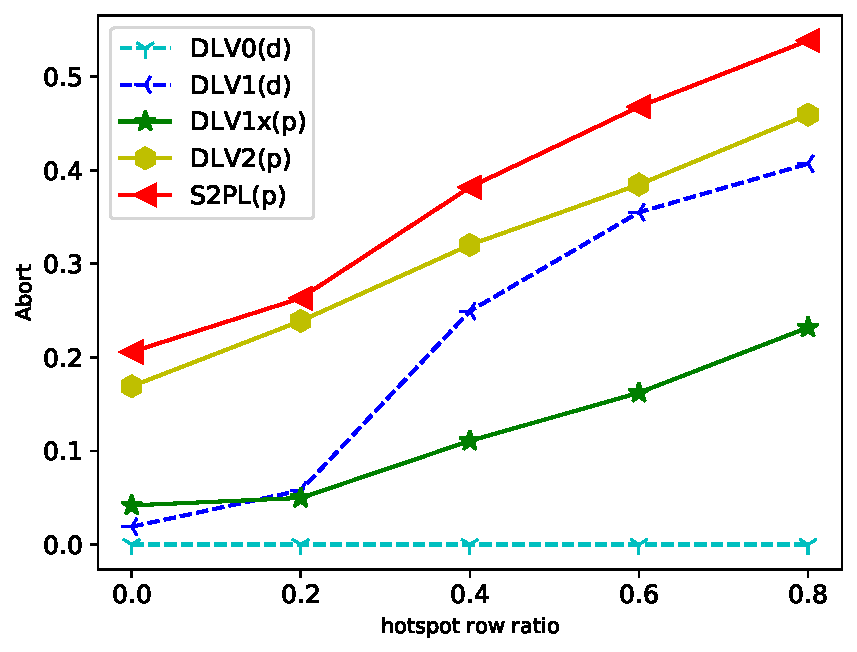
\includegraphics[scale=0.25]{plot_tpcc_hotitem_g_o_abort} \label{fig:plot_tpcc_neworder_add_HotItem_HotItem_gather:abort}
      \captionsetup[subfigure]{margin={0cm,0cm}}
      }
      \caption{Impact of Hot Spot(TPC-C) }
      \label{fig:plot_tpcc_neworder_add_HotItem_HotItem_gather}
\end{figure}



In TPC-C experiments, we first fixed the client number of every shard to 100 and varied the warehouse number between 10 to 60.
Fig.~\ref{fig:plot_tpcc_neworder_add_Warehouse_Warehouse_gather} gives the results.
Then, we fixed the number of warehouses to 40 and varied the percent of the transactions accessing hot tuples(There were 4 hot tuples in total.).
Fig.~\ref{fig:plot_tpcc_neworder_add_HotItem_HotItem_gather} shows the results.

From Fig.~\ref{fig:plot_tpcc_neworder_add_Warehouse_Warehouse_gather} and
Fig.~\ref{fig:plot_tpcc_neworder_add_HotItem_HotItem_gather},
we can see that contention had a big impact on performance. When the degree of contention decreased, the throughput rose quickly.
The DLVs performed better than S2PL in general, as lock violation had shortened their lock blocking time, especially when the degree of contention is high.
However, the different DlVs demonstrated different performance characteristics. 
While DLV0 and DLV1 performed well when there is less contention, their performance dropped when the contention intensified.
This is because contention increases their chance of encountering deadlocks.
In contrast, DLV1x outperformed the other approaches constantly, as it was less affected by deadlocks and abort.


\begin{figure}[tbp]
  \centering
  \captionsetup[subfigure]{margin={0cm,0cm}}
  \subfloat[YCSB TPM]
      { 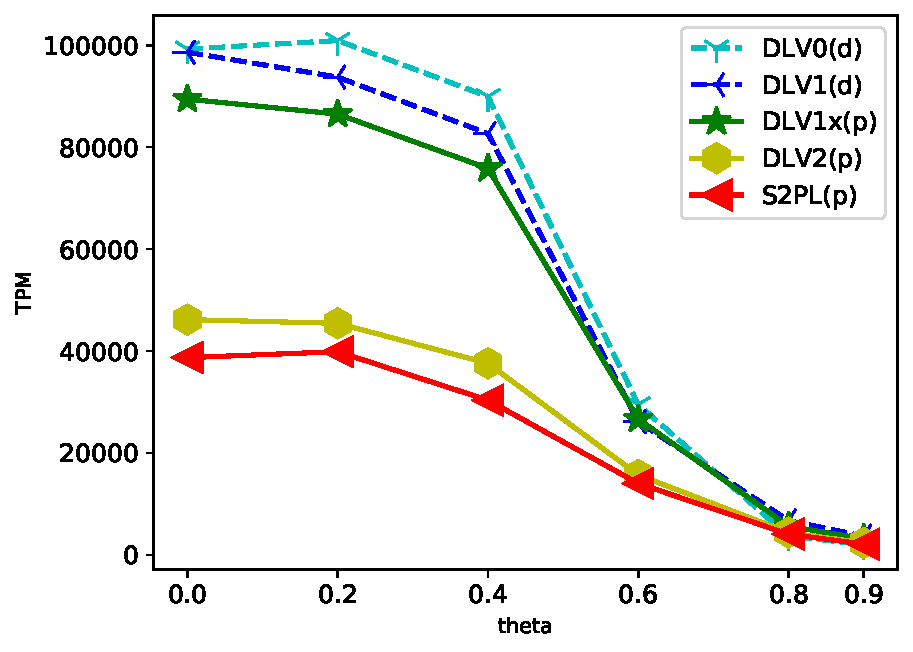
\includegraphics[scale=0.25] {plot_ycsb_theta_g_o_tpm} \label{fig:plot_ycsb_add_Theta_Theta_TPM_gather:tpm}
      
      \captionsetup[subfigure]{margin={0cm,0cm}}
      
      }
      \subfloat[YCSB abort rate]
      { 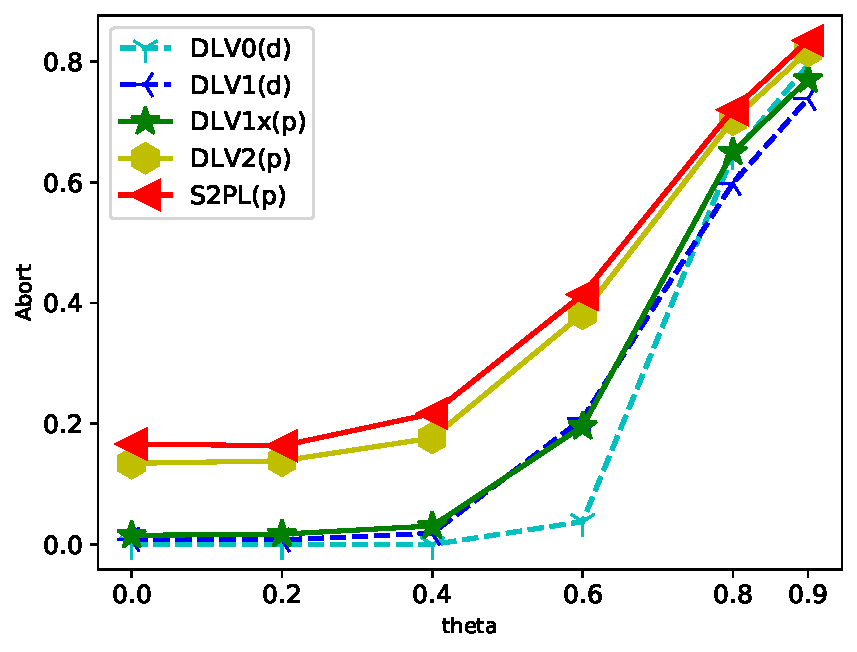
\includegraphics[scale=0.25]{plot_ycsb_theta_g_o_abort} \label{fig:plot_ycsb_add_Theta_Theta_TPM_gather:abort}
      \captionsetup[subfigure]{margin={0cm,0cm}}
      }
      \caption{Impact of Theta (YCSB) }
      \label{fig:plot_ycsb_add_Theta_Theta_TPM_gather}
\end{figure}



In the experiments on YCSB, we fixed the number of clients of every shard to 100.
Then we varied the parameter \emph{theta} (the skewness of the Zipfian distribution) to control the degree of contention.
The larger the \emph{theta}, the more skewed the distribution and the higher the degree of contention.
Fig. ~\ref{fig:plot_ycsb_add_Theta_Theta_TPM_gather} shows how the throughput was affected by the changing skewness.
The results also show that contention had a huge impact on performance.
Similar to the results on TPC-C, DLVs outperformed S2PL.
However, different from the results on TPC-C, DLV0 and DLV1 performed as well as DLV1x in YCSB.
This can be attributed to the characteristics of YCSB. As the data and transactions of YCSB are much simpler than TPC-C, DLV0 and DLV1 will be less affected by deadlocks.

\subsection{On Scalability}

We conducted experiments in both the gathered mode and the scattered mode to evaluate distributed transactions' scalability.
In the gathered mode, all the replica leaders are in the same AZ.
The gathered mode is the most common mode, in which servers in the leaders' AZ served the requests mainly, and servers in other AZs are only for the replication purpose.
In the scattered mode, the replica leaders may spread across different AZs.
Large-scale Web applications usually adopt this mode, which makes their service globally available.

We conducted experiments on the TPC-C workload.
Fig. ~\ref{fig:new_order_add_terminal_gathered} shows the performance of distributed transactions on TPC-C workload in the gathered mode.
We fixed the number of warehouses to 40.
Then we gradually increased the number of clients until the system was saturated.
We can see that DLVs outperformed S2PL in general.
The maximum throughput S2PL could achieve around 31,000 TPM (Transactions per Minute),
while the throughput of DLV1x could achieve 59,000 TPM.


Fig. ~\ref{fig:new_order_add_terminal_scattered}  shows the TPC-C evaluation results in the scattered mode.
As the intra-transaction communication in the scattered mode needs to cross AZs, its performance was slightly worse than that of the gathered mode.
Nevertheless, the results exhibit the same trend. DLVs outperformed S2PL significantly.

Among all the variants of DLV, DLV1x demonstrated the most constant performance.

\begin{figure}[tbp]
  \centering
  \captionsetup[subfigure]{margin={0cm,0cm}}
  \subfloat[NewOrder TPM]
      { 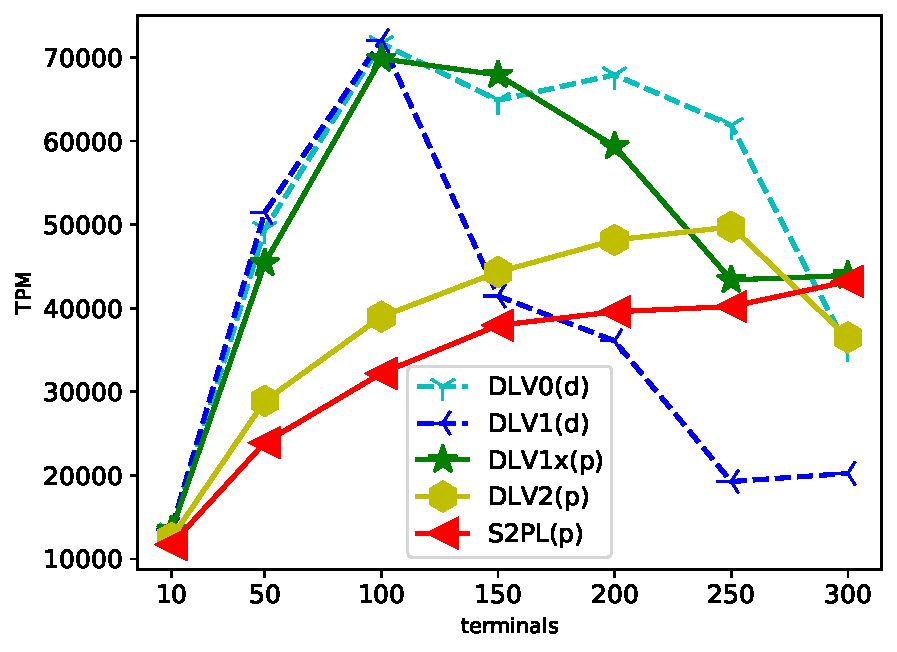
\includegraphics[scale=0.25] {plot_tpcc_terminal_g_o_tpm} \label{fig:new_order_add_terminal_gathered:tpm}
      
      \captionsetup[subfigure]{margin={0cm,0cm}}
      
      }
      \subfloat[NewOrder abort rate]
      { 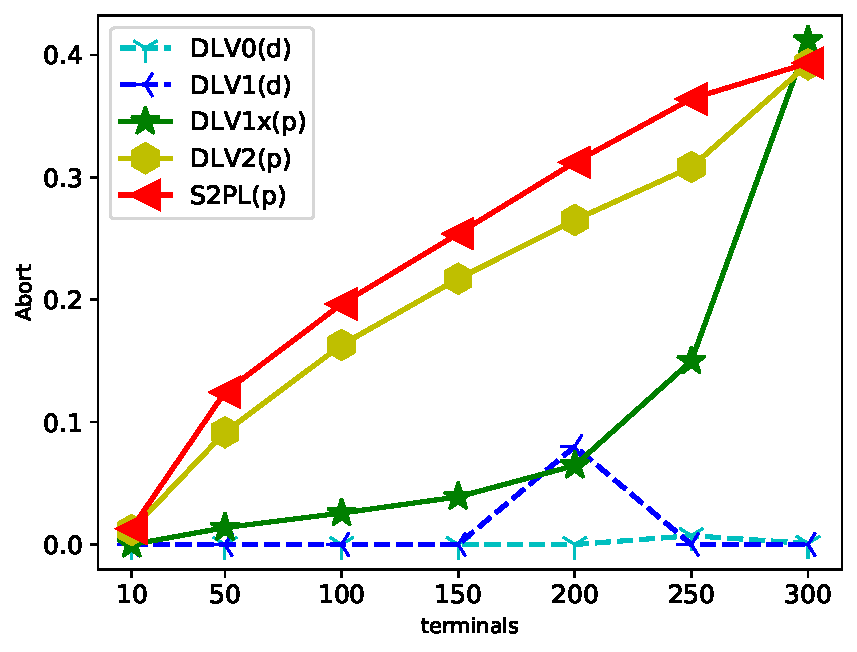
\includegraphics[scale=0.25]{plot_tpcc_terminal_g_o_abort} \label{fig:new_order_add_terminal_gathered:abort}
      \captionsetup[subfigure]{margin={0cm,0cm}}
      }
      \caption{Performance in Gathered Mode (TPC-C) }
      \label{fig:new_order_add_terminal_gathered}
\end{figure}




\begin{figure}[tbp]
  \centering
  \captionsetup[subfigure]{margin={0cm,0cm}}
  \subfloat[NewOrder TPM]
      { 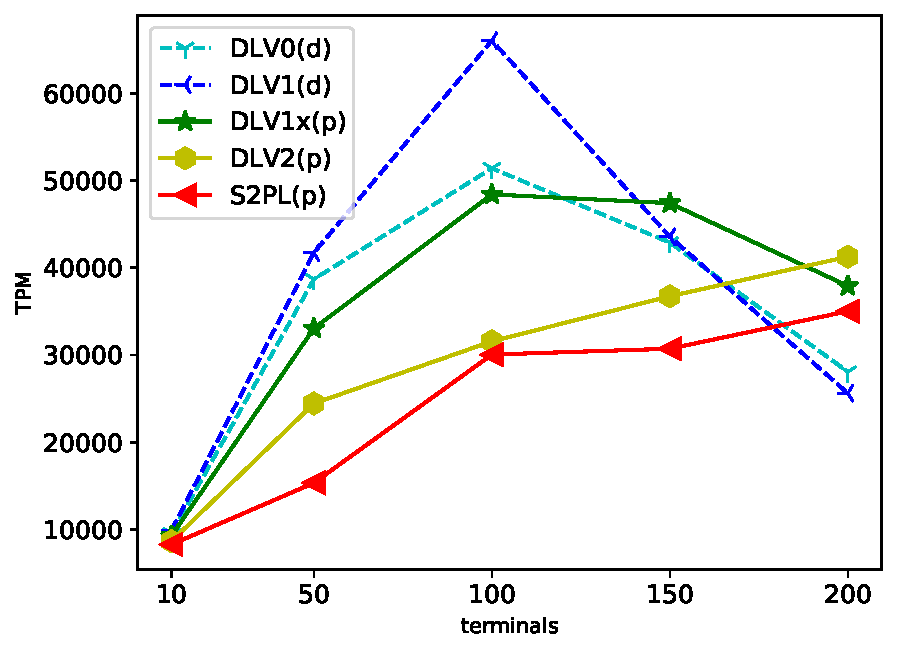
\includegraphics[scale=0.25] {plot_tpcc_terminal_s_o_tpm} \label{fig:new_order_add_terminal_scattered:tpm}
      
      \captionsetup[subfigure]{margin={0cm,0cm}}
      
      }
      \subfloat[NewOrder abort rate]
      { 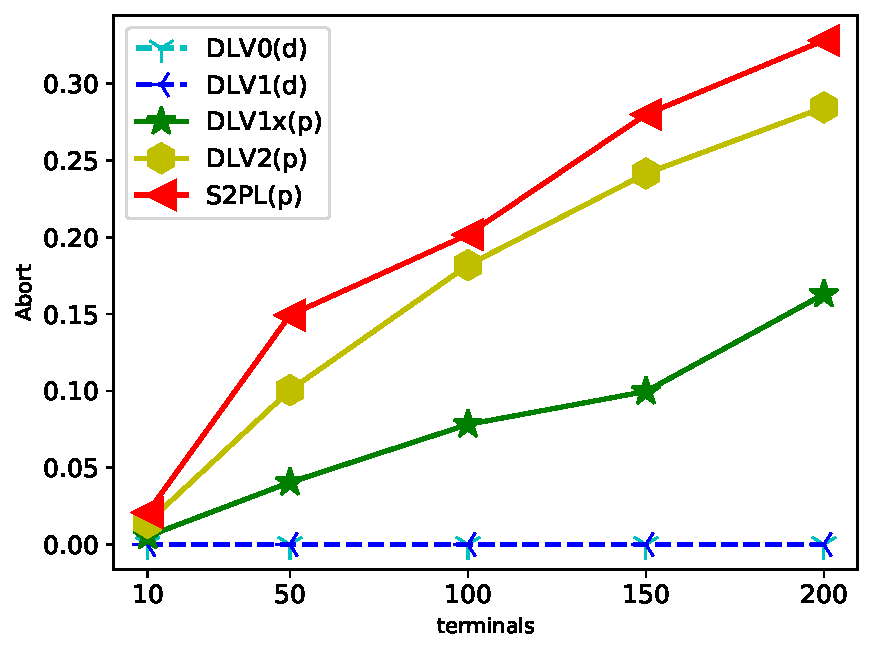
\includegraphics[scale=0.25]{plot_tpcc_terminal_s_o_abort} \label{fig:new_order_add_terminal_scattered:abort}
      \captionsetup[subfigure]{margin={0cm,0cm}}
      }
      \caption{Performance in the Scattered Mode (TPC-C) }
      \label{fig:new_order_add_terminal_scattered}
\end{figure}



\subsection{Evaluation of Interactive Transactions}

%\begin{highlighted}
%change begin

To evaluate the performance of the lock violation on interactive transactions,
we conducted an additional set of experiments on TPC-C, in which each transaction's ${TM}$ interactively accesses data and then enforces a two-phase commit.
Fig \ref{fig:interactive_evaluation} shows the results of increasing hot spot rows.
As mentioned earlier, most interactive transactions are DP transactions.
A DP transaction is determined to be prepared when the \emph{RM}s receive the prepare message.
Therefore, DLV1x performed as well as DLV1 in the experiments, as it can enable lock violation as early as DLV1.
%\end{highlighted}

\begin{figure}[tbp]
  \centering
  \captionsetup[subfigure]{margin={0cm,0cm}, justification=centering}
  \subfloat[TPCC interactive transactions TPM]
    { 
      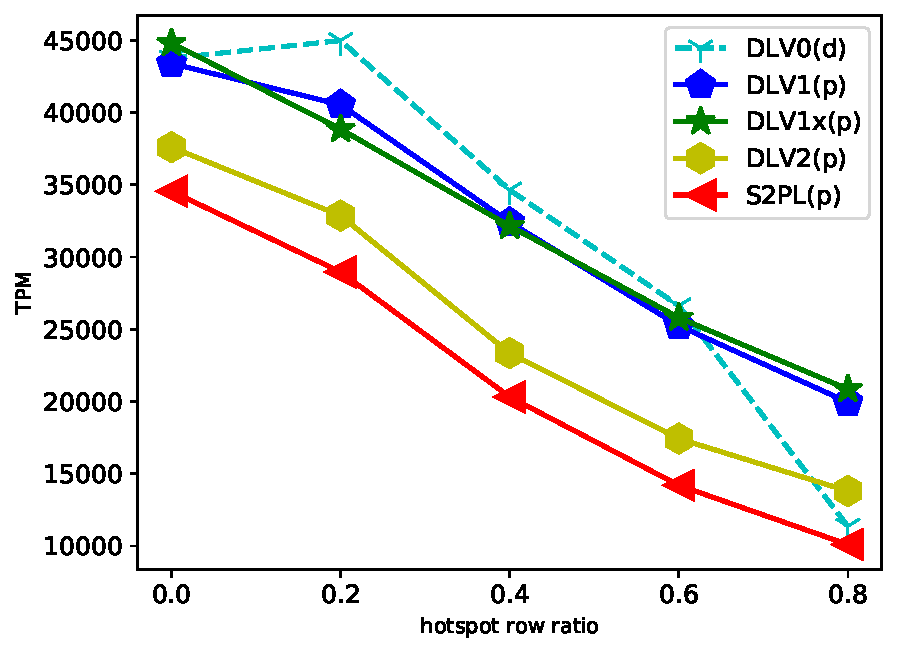
\includegraphics[scale=0.245] {plot_tpcc_hotitem_g_i_tpm} \label{fig:tpcc_add_terminal_interactive:tpm}
      \captionsetup[subfigure]{margin={0cm,0cm}}
    }
    \subfloat[TPCC interactive transactions abort rate]
    { 
      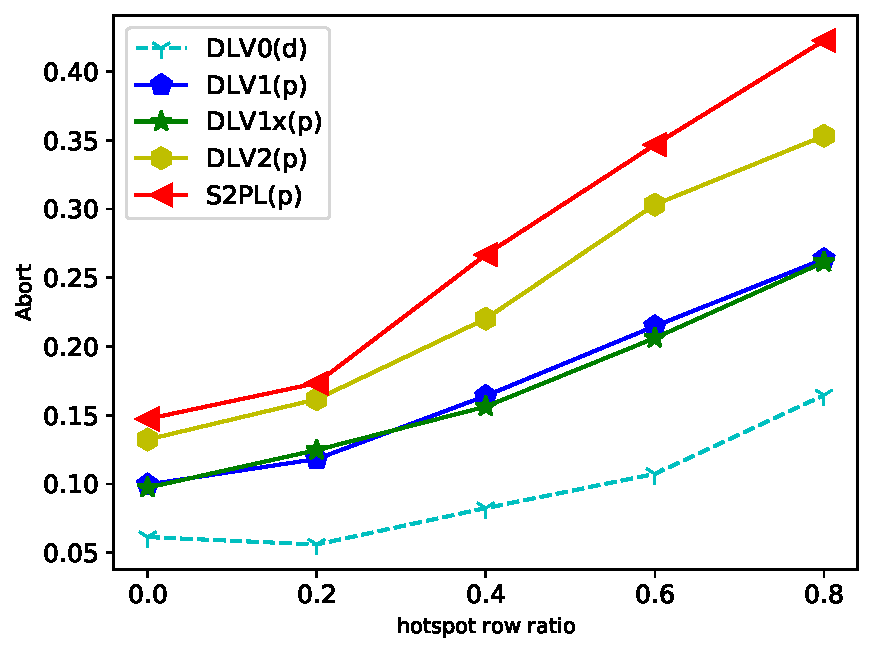
\includegraphics[scale=0.245]{plot_tpcc_hotitem_g_i_abort} \label{fig:tpcc_add_terminal_interactive:abort}
      \captionsetup[subfigure]{margin={0cm,0cm}}
      }
    \caption{TPCC interactive transaction evaluation}
    \label{fig:interactive_evaluation}
\end{figure}



\subsection{Evaluation of Cascade Abort}
%\begin{highlighted}
DLV suffers from cascade abort. In comparison, early lock violation is more vulnerable to cascade abort than
late lock violation.
To evaluate the cost of cascade abort on different lock violation approaches, we conducted additional experiments on TPC-C, in which the number of warehouses was fixed to 40  and the terminal number to 200.
We only considered and evaluated the effect of deterministic abort.

Fig.\ref{fig:evaluation_cascade_abort} shows the cascade abort rate in comparison with the total abort rate.
Fig.\ref{fig:evaluation_cascade_abort:nonexist_row}
shows the abort rates under normal TPC-C workload.
Fig.\ref{fig:evaluation_cascade_abort:nonexist_row} 
shows the abort rates under a modified TPC-C workload, in which each transaction has 10\% of the chance to access a non-existent row and incur an abort. 
 
As we can see, S2PL, DLV2, and DLV1x seldom encounter cascade aborts, no matter whether deadlock detection or deadlock prevention is applied. 
In contrast, there is a significant chance of cascade abort for DLV1 and DLV0, especially when deadlock detection is applied. Deadlock prevention encounters fewer cascade aborts because it tends to abort transactions earlier before cascade abort kicks in. The total abort rates incurred by deadlock prevention were always higher than those by deadlock detection.

%\end{highlighted}

\begin{figure}[tbp]
  \centering

  \captionsetup[subfigure]{margin={0cm,0cm},justification=centering}
  \subfloat[\small no transactions access non-exist rows]
      { 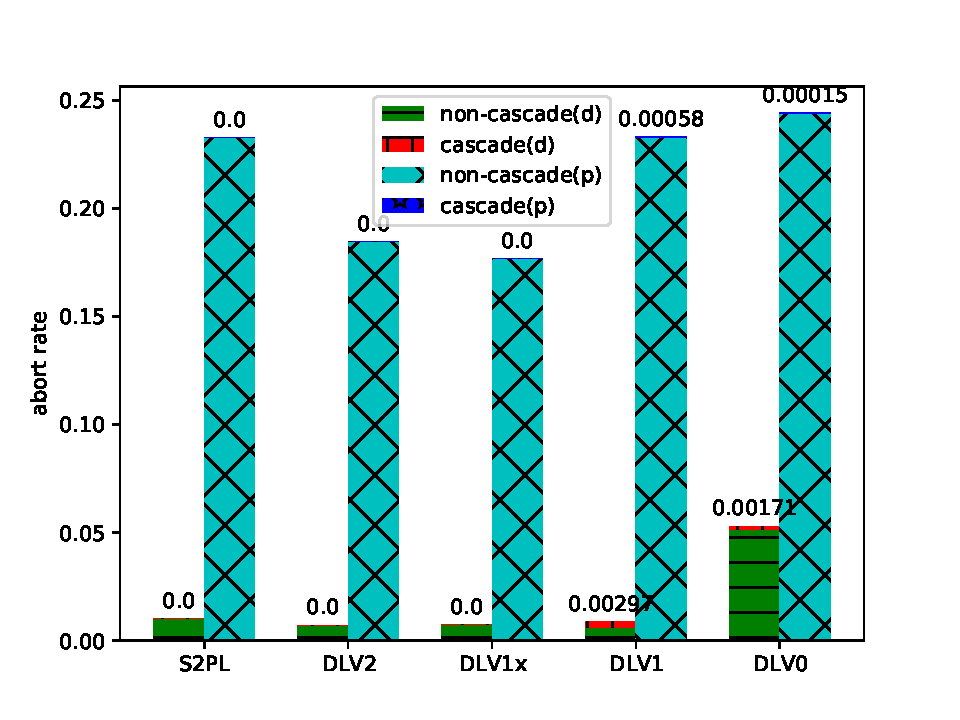
\includegraphics[scale=0.25] {plot_cascade_0.pdf} \label{fig:evaluation_cascade_abort:without_nonexist_row}

      \captionsetup[subfigure]{margin={0cm,0cm}}
      }
  \subfloat[\small 10\% transactions access  non-exist rows]
      { 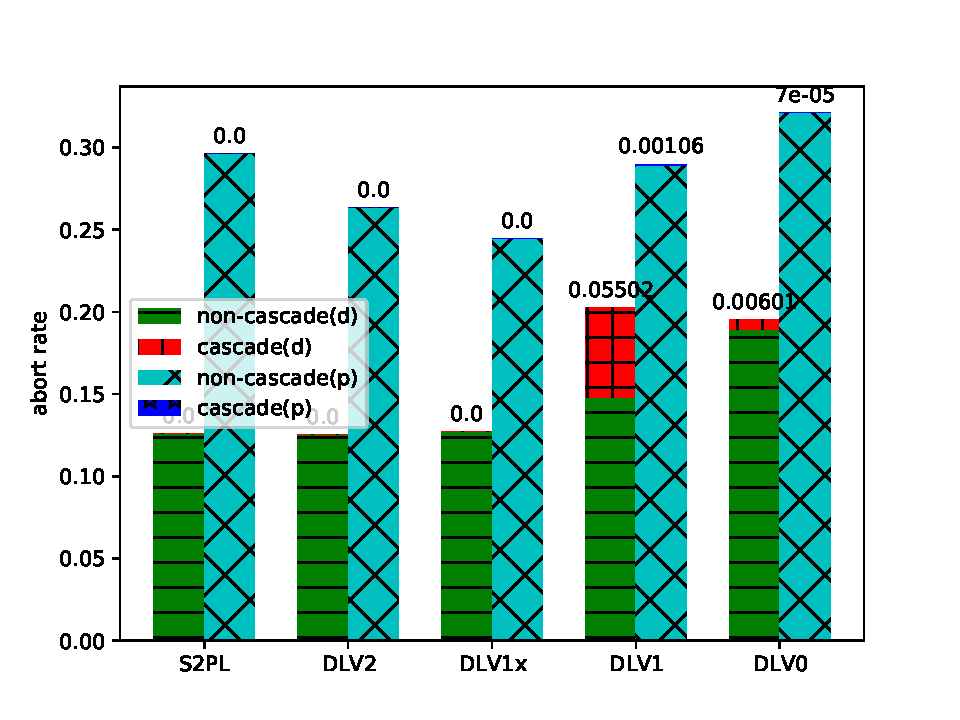
\includegraphics[scale=0.25]{plot_cascade_10.pdf} \label{fig:evaluation_cascade_abort:nonexist_row}
      \captionsetup[subfigure]{margin={0cm,0cm}}
      }

\caption{Cascade abort ratio, \emph{(d)} stands  for deadlock detection, and \emph{(p)} stands for deadlock prevention}
\label{fig:evaluation_cascade_abort}
\end{figure}



\subsection{Evaluation of Transaction Latency}


\begin{figure}[tbp]
  \centering

  \captionsetup[subfigure]{margin={0cm,0cm},justification=centering}
  \subfloat[deadlock detection]
      { 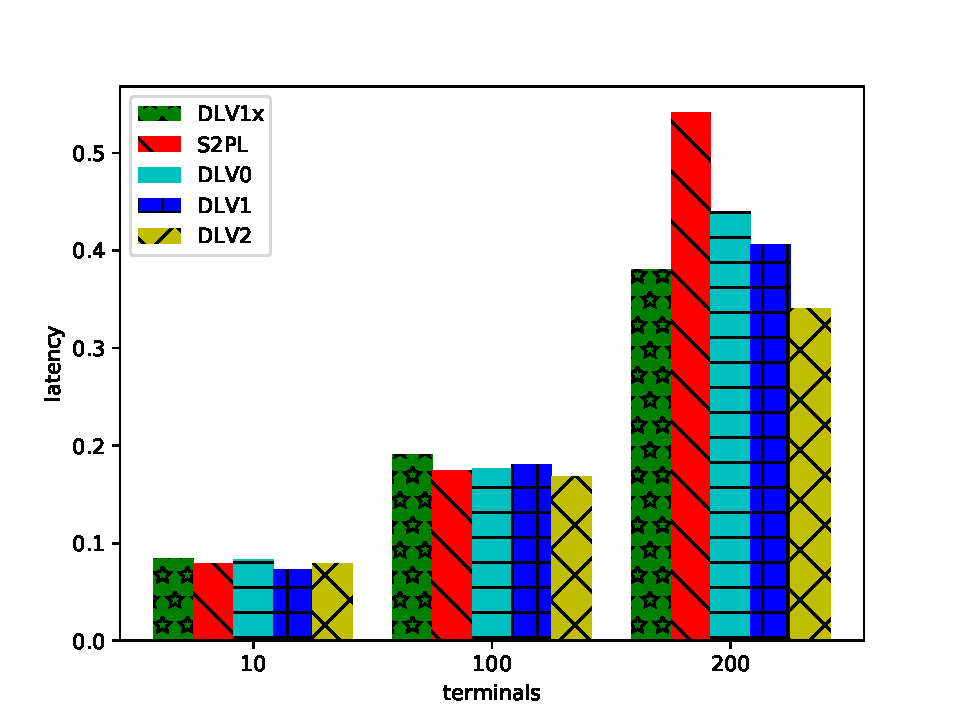
\includegraphics[scale=0.25] {tpcc_neworder_add_Terminal_latency_Detection.pdf} \label{fig:evaluation_latency:deadlock_detection}
      }
  \subfloat[deadlock prevention ]
      { 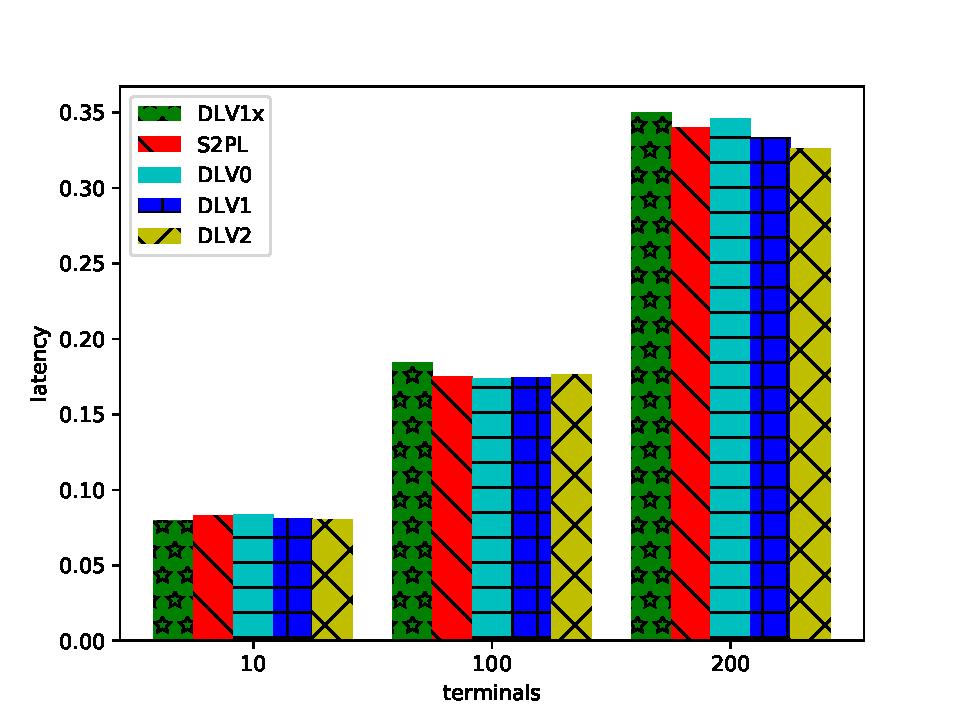
\includegraphics[scale=0.25]{tpcc_neworder_add_Terminal_latency_WaitDie.pdf} \label{fig:evaluation_latency:deadlock_prevention}}

\caption{Transaction Latency(specified in seconds)}
\label{fig:evaluation_latency}
\end{figure}

%\begin{highlighted}
  DLV does not have a direct impact on transaction latency.
  Although DLV can reduce the chance of blocking, a transaction still has to wait for all its preceding transactions to finish before it can commit.
  We conducted a set of experiments to profile the transaction latency of different DLV approaches on TPC-C. 
  In the experiments, the TPC-C warehouse number was fixed to 40, and the terminal number was set to 10, 100, and 200, respectively.
  During the experiments, a transaction would be immediately retried after it was abort.
  The average execution time of committed transactions was calculated as the transaction latency. The results are shown in Fig. \ref{fig:evaluation_latency}.
  
  We can see that the transaction latency is mainly affected by the deadlock handling cost and the workload.
  In general, deadlock prevention incurs less overhead and results in better latency than deadlock detection. If we increase the workload, the latency can grow quite rapidly.
  In contrast, if the same deadlock handling method is applied and the workload is fixed, the average transaction latencies of different approaches are actually similar. 

%\end{highlighted}
\iffalse
\subsection{Non-availability Time After Failure}


\begin{figure}[tbp]
  \centering
  \captionsetup[subfigure]{margin={0cm,0cm}}
  { 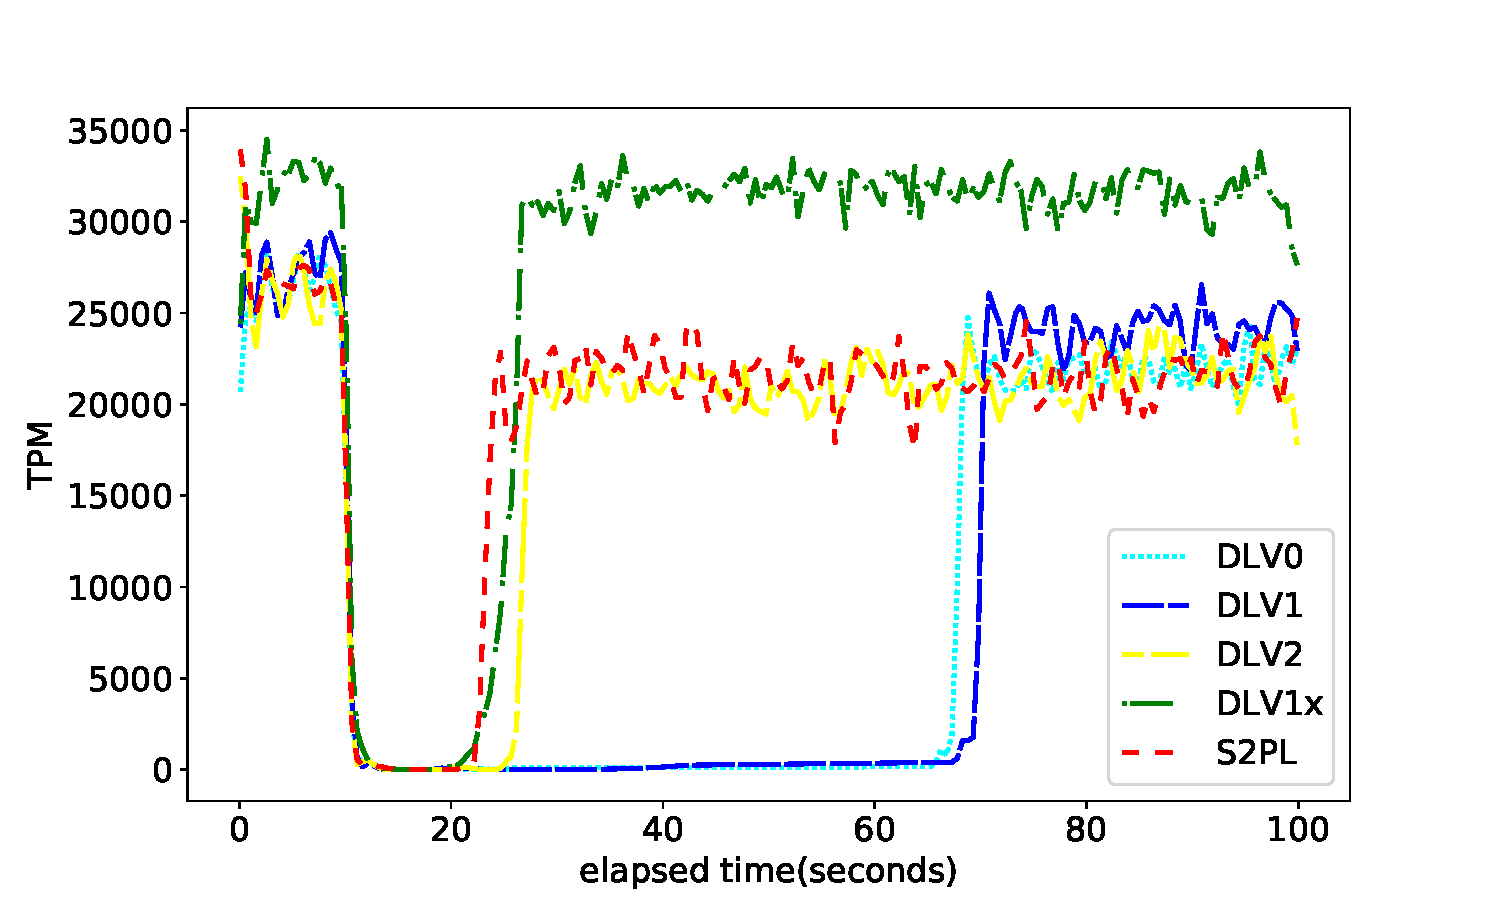
\includegraphics[scale=0.28] {plot_availability}
  \caption{non availability time after one AZ is down}
  \label{fig:plot_availability:tpm}}
\end{figure}


Due to cascade abort, a GDDB may take more time to restart when a failure occurs.
In our final set of experiments, we evaluated the non-availability time of the different approaches when encountering an AZ failure.
Fig~\ref{fig:plot_availability:tpm} shows how throughput changes over time elapsed during one AZ failure.
This result shows DLV0, DLV1 endures longer non-available time after an AZ failure.
DLV2 and DLV1x have less non-available time. This is because late lock violation faces less cascade abort.
\fi

\subsection{Experimental Conclusion}

In conclusion, our experimental evaluation showed that the geo-replication could have a big negative impact on distributed transactions' performance.
Besides the overheads of data synchronization incurred by replication, the prolonged lock blocking time is a main contributor to the degraded performance.
We demonstrated that lock violation could be an effective measure to shorten the critical lock time and boost the performance of GDDB.
However, it is important to find the right time to violate the locks to harness the benefit of lock violation.
For different timing of lock violation, different approaches should be adopted for handling deadlocks.
Our evaluation also showed that late lock violation could be superior to early lock violation in most cases, as it has less abort and works well with lock prevention, which is less expensive than distributed lock detection.


\section{Conclusion}
\label{sec:conclusion}

This paper discussed the application of lock violation in geo-replicated distributed databases.
Lock violation is not only concerned with the concurrency control mechanism, but it is also related to the modules of recovery and persistence.
Therefore, its adoption requires a holistic redesign of the transaction processor.
In this paper, we proposed such a holistic design and conducted experiments to evaluate its effectiveness.
The results showed that lock violation could boost the performance of a geo-replicated distributed database, especially when the degree of contention is high.
Moreover, we found that not all lock violation approaches can be beneficial. We identified the right design of lock violation to maximize its effects.

%\begin{highlighted}

DLV cannot reduce transactions' latencies, while it enables better throughputs.
It can consolidate the wait of transaction execution, especially that in the commit phase.
When there is more idle resource, it is more rewarding to use aggressive lock violation as well as deadlock detection to precisely avoid false-positive abort.
In contrast, when a system reaches its saturation point, the system should switch to a more conservative
lock violation to avoid its overheads.
Deciding opportunities to conduct DLV can be an interesting topic for future work.


\section*{Acknowledgment}
We want to thank the anonymous reviewers for the valuable comments in helping improve the paper.


\bibliographystyle{reference/IEEEtran}
\bibliography{reference/IEEEexample}


\end{document}

